\documentclass[txfonts]{NSTexam}
\showanswerstrue
%git clone https://git.overleaf.com/61e43e46c2ac07e4711f8acf
\noversion

%\documentclass{article}
%\documentclass{article}
\usepackage[utf8]{inputenc}
\usepackage{amsmath}
\usepackage{bbm}
\usepackage{xcolor}
\usepackage{afterpage}
%\usepackage{tikz}
\usepackage{cancel}
%\usepackage[compat=1.0.0]{tikz-feynman}
%
\newcommand{\bookwork}[1]{{\bf BOOKWORK[ #1 ] }}

\usepackage{tikz}
\usetikzlibrary{trees}
\usetikzlibrary{decorations.pathmorphing}
\usetikzlibrary{decorations.markings}


  \definecolor{jblue}  {RGB}{20,50,100}
  \definecolor{lblue}  {RGB}{40,100,240}
  \definecolor{npurple}  {RGB} {153, 51, 204}
  \definecolor{wred}   {RGB}{217,0,56}
  \definecolor{white}   {RGB}{255,255,255}
  
  \definecolor{korange}   {RGB}{235, 80,  43}
  \definecolor{korange2}   {RGB}{245, 100,  63}
  \definecolor{kyelloworange}   {RGB}{255, 210,  110}
  \definecolor{kyelloworange2}   {RGB}{240, 170,  90}
  \definecolor{kred}   {RGB}{204,  102, 153}
  \definecolor{kpurple}   {RGB}{153,  61, 190}
  \definecolor{kpurplelight}   {RGB}{213,  161, 230}

          % Define styles for the different kind of edges in a Feynman diagram
  \tikzset{
    photon/.style={decorate, decoration={snake}, draw=npurple,very thick},
    boson/.style={decorate, decoration={snake}, draw=npurple,very thick},
    electron/.style={draw=jblue,very thick, postaction={decorate},
             decoration={markings,mark=at position .55 with {\arrow[draw=jblue]{>}}}
    },
    electron2/.style={draw=jblue,very thick, postaction={decorate},
             decoration={markings,mark=at position .55 with {\arrow[draw=jblue]{<}}}
    },
    fermion/.style={draw=jblue,very thick, postaction={decorate},
              decoration={markings,mark=at position .55 with {\arrow[draw=jblue]{}}}
    },
    gluon/.style={decorate, draw=korange,very thick, %kred
      decoration={coil,amplitude=4pt, segment length=6pt}},
    higgs/.style={draw=wred,very thick, postaction={decorate},
             decoration={markings,mark=at position .55 with {\arrow[draw=wred]{>}}}
    },
    nothing/.style={draw=white,very thick}
  }




\usepackage{hyperref}

\newcommand\fra{\frac{|\vec p|}{E+m}}
\newcommand\expi{e^{i\phi}}

\newcommand\hide[1]{{}}
\newcommand\ANS[1]{{

\answer % For some reasons need \begin{answer}\end{answer} on overleaf, but \answer\endanswer on my mac


{\color{blue}
#1
}
 
\endanswer

}}

\newcommand\POSTMARKING[1]{{

{\color{magenta}
[\textbf{NOTE ADDED POST MARKING:}

#1
]
}
}}

\newcommand\alig[1]{{\begin{align}#1\end{align}}}
\newcommand\com[2]{{
\left[#1,#2\right]
}}
\newcommand\anticom[2]{{
\left\{#1,#2\right\}
}}
\newcommand\unit{
\mathbbm{1}
}
\newcommand\matTwoTwo[4]{
\left(\begin{array}{cc}
#1 & #2 \\ #3 & #4
\end{array}\right)
}
\newcommand\vecTwo[2]{
\left(\begin{array}{c}
#1 \\ #2 
\end{array}\right)
}
\newcommand\vecFour[4]{
\left(\begin{array}{c}
#1 \\ #2 \\ #3 \\ #4 
\end{array}\right)
}

%\title{Notes}
%\author{kesterlester }
%\date{November 2020}

\begin{document}

\tripos{NATURAL SCIENCES TRIPOS Part II} 
%\tripos{NATURAL SCIENCES TRIPOS:\qquad Part III Astrophysics} 
%\tripos{MASTER OF ADVANCED STUDY IN PHYSICS} 
%\tripos{{\color{red}[Are there too many or too few triposes and courses listed above?]}}
\date{Friday 3rd June 2022 \qquad 09:00 to 11:00} % TIME ADAPTED LAST MINUTE FOR CORONAVIRUS REASONS
%\date{Tuesday 19th January 2021 \qquad 14:00 to 16:00} % ORIGINAL DATE NAND TIEM
\paper{PHYSICS (6)}
\paper{PHYSICAL SCIENCES: HALF SUBJECT PHYSICS (6)}
\paper{\phantom{MOO}}
\paper{PARTICLE AND NUCLEAR PHYSICS}
\begin{rubric}Candidates offering this paper should attempt a total of \textbf{five} questions: all \textbf{three} questions from Section A and \textbf{two} questions from Section B.

\vspace{0.8 cm}
\framebox[0.83\columnwidth]{\begin{minipage}{0.8\columnwidth}
As in the presentation in lectures, natural units of $\hbar = c = \mu_0 = \epsilon_0 = 1$ are used throughout this paper.
\end{minipage}}
\vspace{0.8 cm}

The approximate number of marks allocated to each question or part of a question is indicated in the right margin. This paper contains 11 sides, including this coversheet, and is accompanied by a handbook giving values of constants and containing mathematical formulae which you may quote without proof.
\end{rubric}

\requirements{$2\times 20$ Page Answer Book\\
%Metric graph paper
Rough workpad\\Yellow master coversheet}{Mathematical Formulae handbook\\Approved calculator allowed} \warning

%\newpage
%\thispagestyle{plain} % empty
%\mbox{}

\clearpage
\newpage

~
\newpage

\thispagestyle{turnover}

\section{A \\ \em Attempt \textbf{all} questions in this Section.  Answers should be concise and relevant formulae may be assumed without proof.}

\begin{questions}

\question
Describe the three main kinds of $\beta$-decay, and the kinematic conditions under which each occurs.   At fixed mass number, $A$, how many isotopes are typically stable with respect to $\beta$-decay and why?
\marks{4}

\ANS{

 [THIS QUESTION IS ENTIRELY BOOKWORK]
 
 
 (i)
 
 $\beta^-$: $n\rightarrow p+e^-+\bar \nu_e$ can happen spontaneously in isolation, or in nucleii ${}^A_Z X \rightarrow {}^A_{Z+1}Y + e^-+\bar\nu_e$ when nuclear masses satisfy $m_X>m_Y+m_e+m_\nu$.
 
 $\beta^+$: $p\rightarrow n+e^++\nu_e$ can happen in nucleii as ${}^A_Z X \rightarrow {}^A_{Z-1}Y + e^-+\bar\nu_e$ when neuclear masses satisfy $m_X>m_Y+m_e+m_\nu$.
 
 $e$-capture: $p+e^-\rightarrow n+ \nu_e$ or ${}^A_Z X + e^- \rightarrow {}^A_{Z-1}Y +\nu_e$ needs nuclear masses $m_X+m_e>m_Y+m_\nu$ if the electron is captured locally from an atom (rather than from a high energy source).
 
 (ii)
 Then need a short description of the main points given by this slide from lectures:
 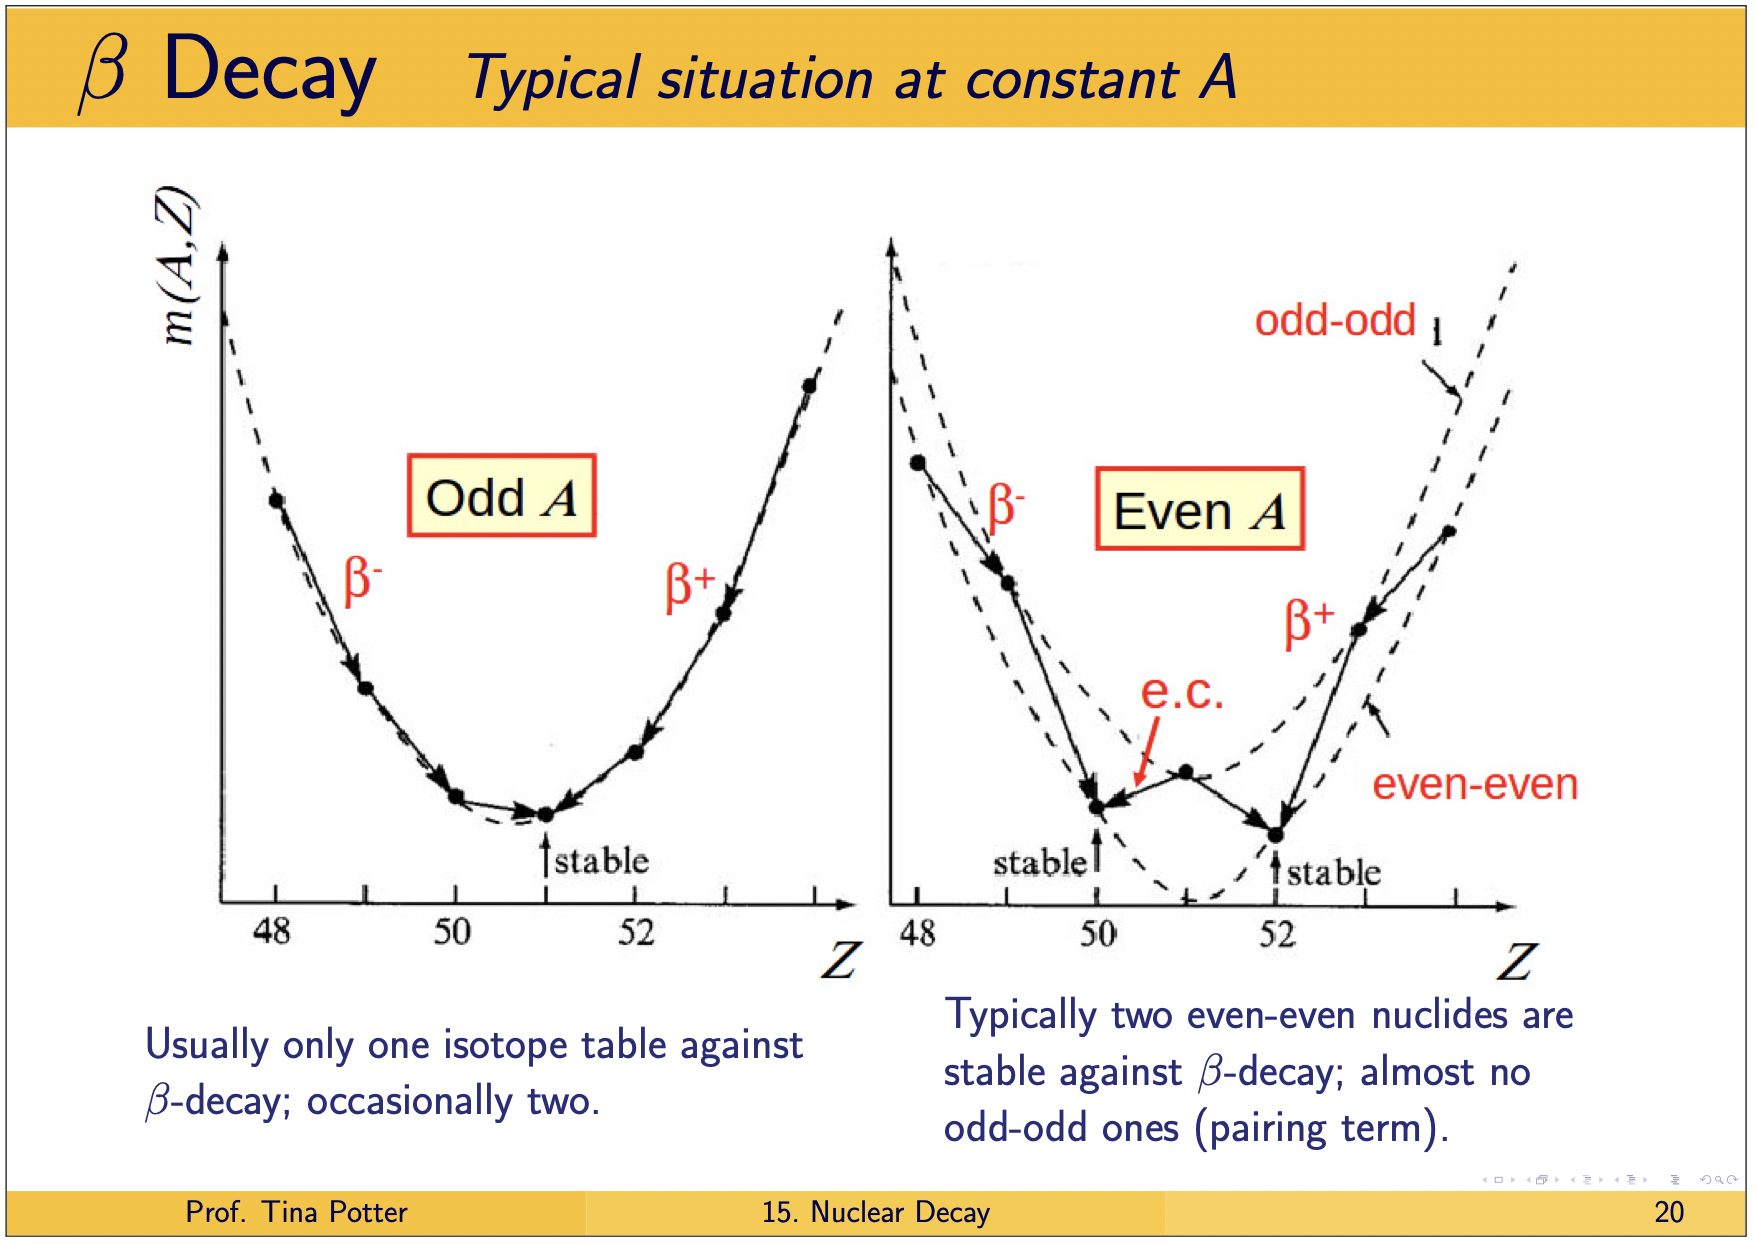
\includegraphics[width=0.8\textwidth]{Images/potter_nuclear_slide_20.png}.
 
 \POSTMARKING{Some candidates interpreted the "three types" as not betaPlus, betaMinus and electron capture but as betaMinus, betaMinus-Gamov-Teller and betaMinus-NthForbidden (or similar).  As the wording of the question didn't exclude this possible interpretation, I marked such candidates generously. However, I also looked carefully at such candidates' answers to the last part of this question to check whether or not they treated the beta-plus decays there as beta decays or not (most scientists consider betaPlus decays to be a form of beta decay). There answer to the last part had to make sense given any answer to the first part for full credit.
 
 Also a small but significant number of candidates, when attempting to describe the kinematic conditions under which each sort of decay could take place used phrases like :
 ``There are three main types of beta decay.
 (i) Beta-minus decay: Nuclei that are rich in neutrons tend to decay by emitting an electron along with an antineutrino; (ii)
 Beta-plus decay: Neutron-deficient nuclei tend to decay by positron emission or electron capture (see below); and (iii)
 Electron capture.''.  Coincidentally this appears to be an almost verbatim copy of the text that google returns when you ask google `what are the three types of beta decay'. I mention this fact neither to accuse any candidates of cheating (I have no reason to believe any candidate cheated!) nor to justify the phrasing of the first part of the question. Instead I mention it as a precursor to explaining why I  did not accept such answer for full credit in relation to the `kinematic conditions' part of this question. The reason I deducted a mark here is that I viewed such answers as tautological or content free. Yes: a decay that rids a nucleus of (say) a neutron could indeed be described as a decay of a neutron-rich nucleus.  But that is more much like saying that people who like cheese are cheese lovers. It doesn't explain the circumstances in which people like cheese. I wanted to see more than that, e.g.~I wanted to see evidence that candidates new which beta decays require a nuclear environment (e.g.~to allow the p to n transition) and which do not, or what conditions are needed on masses or energies, etc.}
 

}

\question
Describe the principles underpinning radio-carbon dating.
\marks{4}

\ANS{

[THIS QUESTION IS ENTIRELY BOOKWORK]

(1) 14N+n to 14C+p in upper atmosphere due to cosmic rays, (2) leads to one part in $10^{12}$ of ${}^{14}$C in atmos, (3) uptake by living organisms until their death, (4) ${}^{14}$C $\rightarrow$ ${}^{14}$N+e+nubar with half life of 5730 years, so (5) measure num decays per second per unit mass (specific decay rate) to infer age since death.  

Lectures noted:
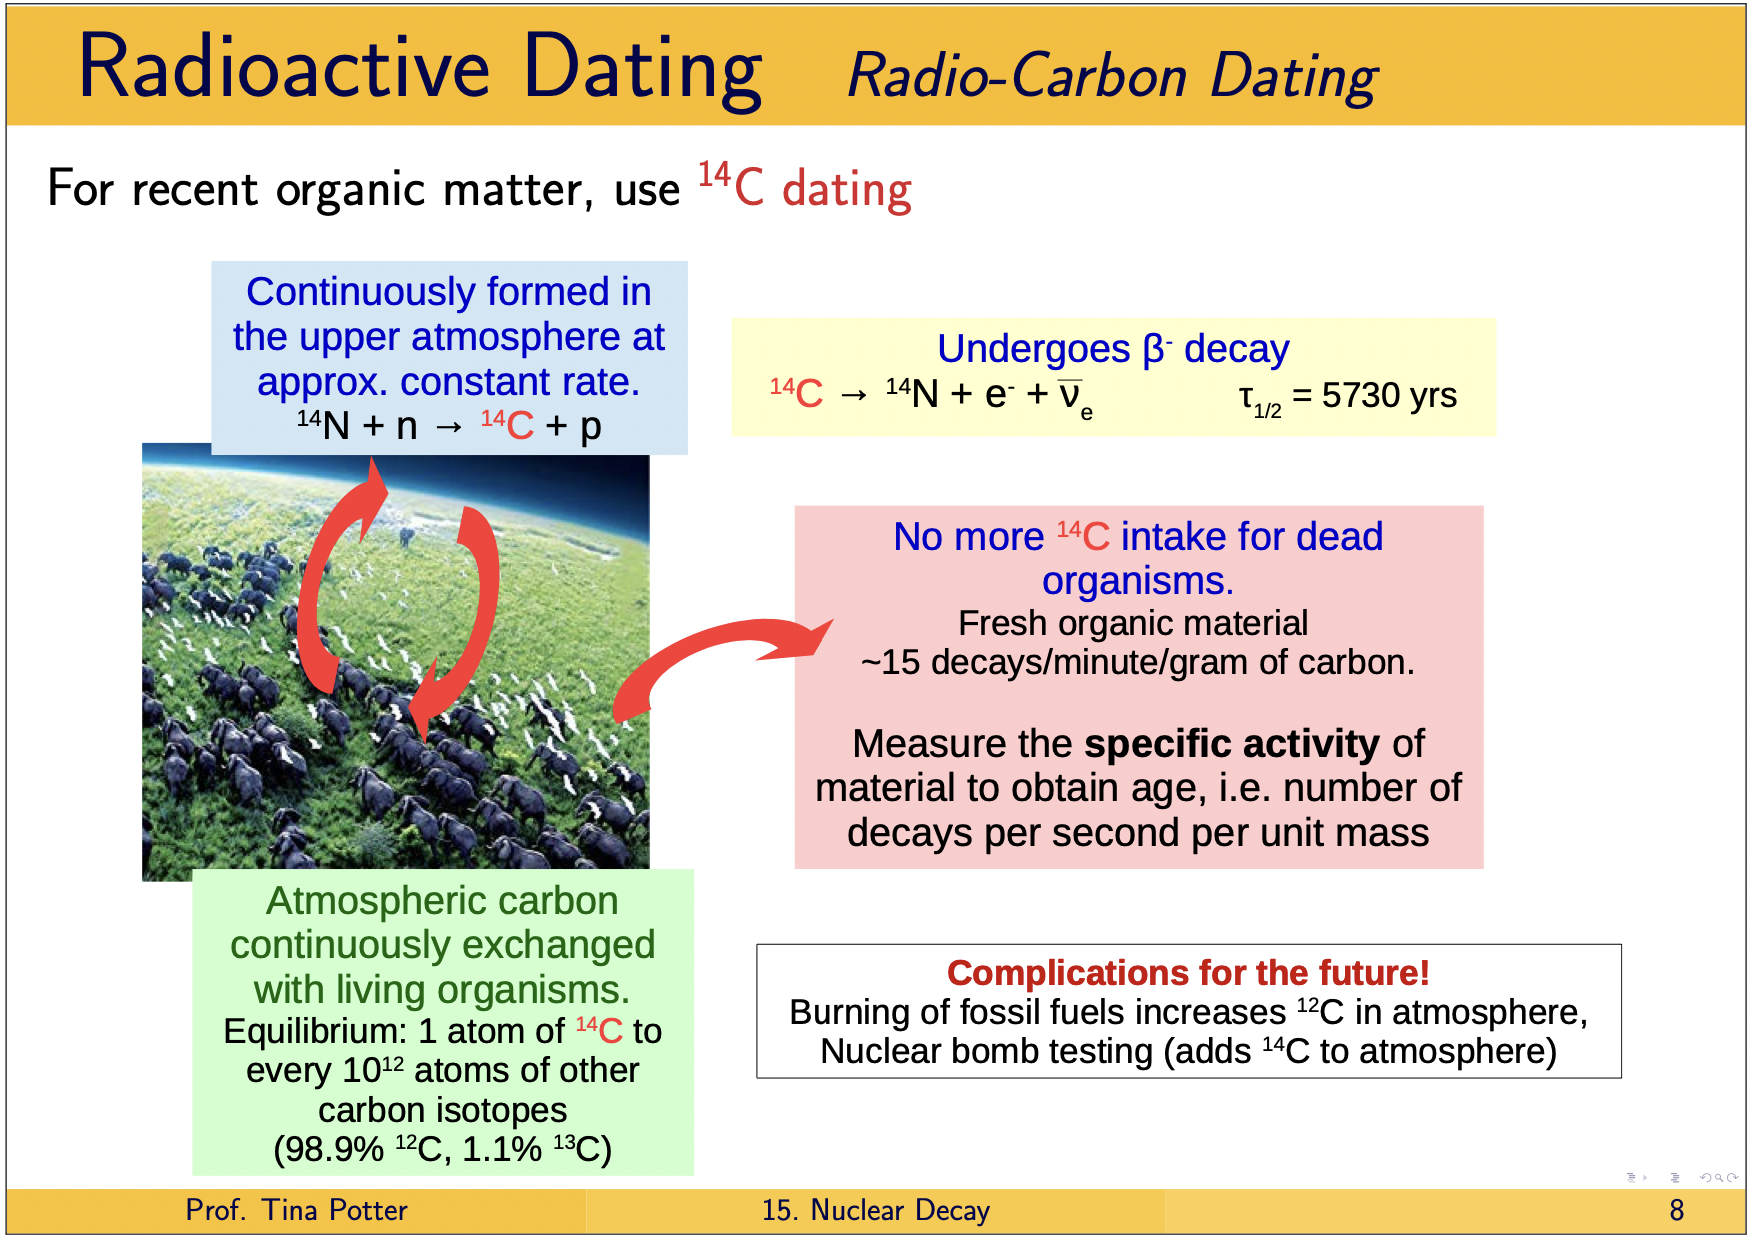
\includegraphics[width=0.8\textwidth]{Images/potter_nuclear_slide_8.png}.

\POSTMARKING{
Mostly this question was well answered, but a significant fraction of candidates lost marks for writing text that appeared to imply that the candidate believed that C14 was only unstable in dead organisms, indicated by phraseology like `Once the organism dies, the C14 nucleii then begin to decay' rather than `Once the animal dies the C14 nucleii in the organism (which have always been decaying) are no longer replenished by exchange with C14 in the atmosphere.' SImilarly, full marks were only awarded when candidates explained (as a significant number did not) why it is that the atmospheric C14 concentration is constant(ish) with time (and constant at a non-zero value) due to cosmic ray production of neutrons and neutron capture. Just saying the atmospheric C14 level is constant and then starts to lower in dead organisms is true but not enough on its own. 
}
}

\question
The Standard Model has four gauge bosons:  $g$, $W$, $Z$ and $\gamma$.  The  Feynman rules of this theory include fundamental vertices which couple together \textbf{only} certain groups of these gauge bosons.  A fundamental vertex of The Standard Model coupling together $N$ gauge bosons (i.e., one having $N$ legs) is called an `$N$-gauge-boson vertex'.
\marks{4}
\begin{parts}
\part
How many two-gauge-boson vertices exist in The Standard Model? If the number is non-zero, draw a picture of each vertex, clearly indicating the type of boson on each leg.
\part
Repeat (a) for three-gauge-boson vertices.
\part
Repeat (a) for four-gauge-boson vertices.
\part
Repeat (a) for five-gauge-boson vertices.
\end{parts}
 
\ANS{
\clearpage

COMMENT ON QUESTION:

This is not supposed to be bookwork `as such' (though it is related) since the way SM vertices are talked about in both this course and in many books is usually very compartmentalised. That is to say that QED vertices will be usually be talked about in one part of the course, and weak vertices in another, etc.  Although every book/lecturer will almost certainly say somewhere that `photons couple only to electric charge' or that `gluons couple only to colour',  it is very rare for a lecturer or a text book to explicitly make a statement like `there is no $g\gamma\gamma$-vertex'. The students should be able to see there is not one (if they don't already know this), but from past experience supervising students in this course I suspect many will not. Similarly, many students seem to have a very vague idea about which gauge-boson self interactions area allowed -- or for that matter whether they are constrained at all.  The point of this question, therefore, is to take the vertices of the SM outside the friendly context of individual sub-theories (like QCD or QCD) and put them into a wider context, so that we can then determine which of the students have (or don't have) a clear/firm idea that there is no $ggZ$-vertex, etc.   The somewhat wordy construction used in the question is there (rather than a free form `just tell me about the vertices which do exist') to make sure that the people answering the question have in mind the full generality of what they are being asked to consider. and can give large answers if they want to. [The brightest of them will, however, rapidly realise that there is very little to do in this question -- which is fine.]
 
 \vspace{1cm}
 
 ANSWER TO QUESTION:
 
 (a)
 There are 0 two-gauge boson interactions in the SM.

 (b)
 There are 3 three-gauge boson interactions in the SM.  The gauge bosons on the legs of each in turn are:
 
1: $ g g g $, 
 
2:  $ W W Z $, 
 
3: $ W W \gamma $.
 
 (c)
 There are 5 four-gauge boson interactions in the SM.  The gauge bosons on the legs of each in turn are:
 
 1: $ g g g g $, 
   
2:  $ W W W W $, 
 
3:  $ W W Z Z $, 
 
4:  $ W W Z \gamma $, 
 
5:  $ W W \gamma \gamma $.
 
 (d)
 There are 0 five-gauge boson interactions in the SM.
 }

\clearpage

%%%%%%%%%%%%%%%%%%%%%%%%%%%%%%%%%%%%%%%%%%%%%%%%%%%%%%%%%%%%%%%%%%%%
%%%%%%%%%%%%%%%%%%%%%%%%%%%%%%%%%%%%%%%%%%%%%%%%%%%%%%%%%%%%%%%%%%%%
%%%%%%%%%%%%%%%%%%%%%%%%%%%%%%%%%%%%%%%%%%%%%%%%%%%%%%%%%%%%%%%%%%%%

\section{B\\\em Attempt \textbf{two} questions from this Section.}

\question

\noindent 
\startpart

\noindent
${}^{23}\mathrm{Ne}$ is unstable.  Over time it converts to ${}^{23}\mathrm{Na}$. Among the products emitted during its decay are photons and these are observed at energies of 
%awk 'BEGIN{g=0;e1=0.440;e2=2.076;e3=2.982; print e1-g, e3-e2,e2-e1,e2-g,e3-e1,e3-g}'
$\gamma_1=0.440~\mathrm{MeV}$, $\gamma_2=0.906~\mathrm{MeV}$, $\gamma_3=1.636~\mathrm{MeV}$, $\gamma_4=2.076~\mathrm{MeV}$, $\gamma_5=2.542~\mathrm{MeV}$ and $\gamma_6=2.982~\mathrm{MeV}$.
\begin{allparts}
\part
By what nuclear process(es) does  ${}^{23}\mathrm{Ne}$ decay to ${}^{23}\mathrm{Na}$ ?\marks{2}


\ANS{

We want the candidates to explain that the neon is initially \textbf{beta} decaying to (possibly though not necessarily) excited states of sodium, and that the excited states are then decaying to the ground state through gamma radiation.  I.e., they need to explain that the diagonal transitions are beta and the vertical transitions are the photons.

\POSTMARKING{Median mark was 1 out of 2 here as more than half of candidates omitted to mention that some ${}^{23}\mathrm{Ne}$ decays to the ${}^{23}\mathrm{Na}$ via beta decay and THEN gamma decay rather than JUST beta decay.}
}
\part
How many energy-level schemes of the form shown below are compatible with the  gamma ray energy spectrum reported?  \shorthint{You should find more than one.}  Draw an energy-level diagram for each scheme that you find, making sure to label on it: (i) which $\gamma_i$ corresponds to which transition, and (ii) the  %numerical 
values taken by the excitation energies $E_1$, $E_2$ and $E_3$.\marks{3}

%\begin{center}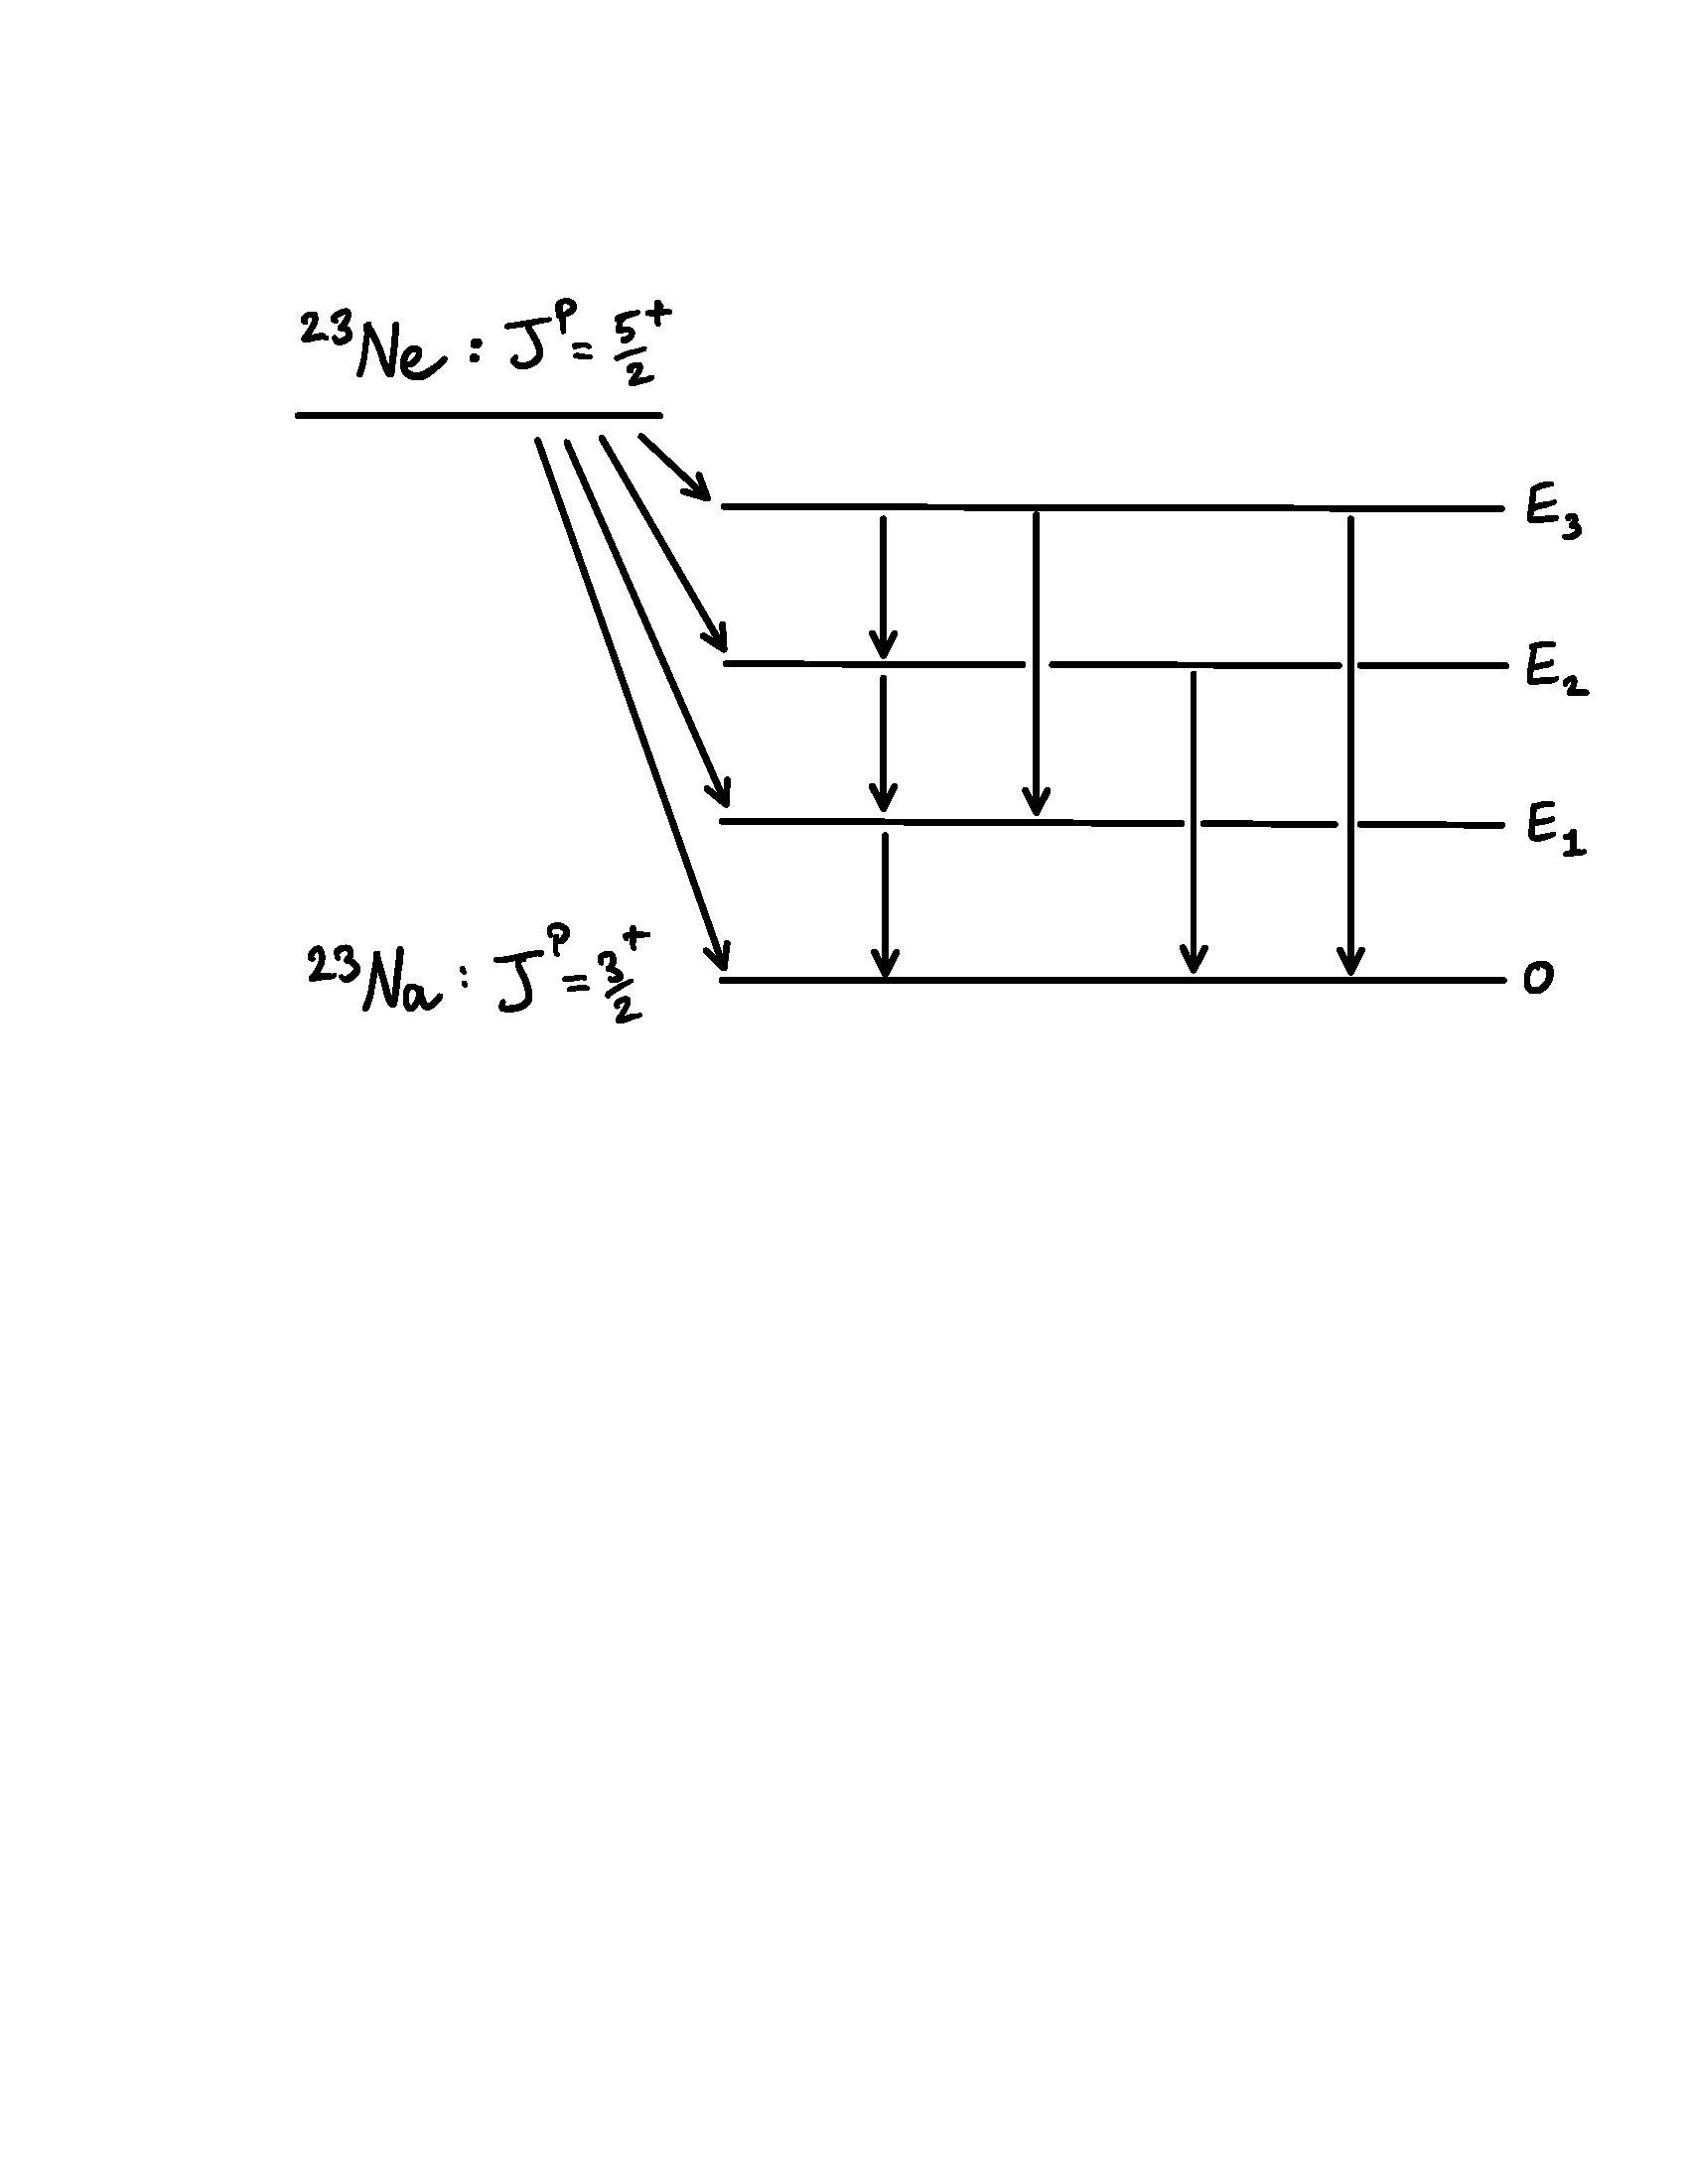
\includegraphics[width=0.65\textwidth]{Images/23Na_energy_levels_ipad.pdf}\end{center}
\begin{center}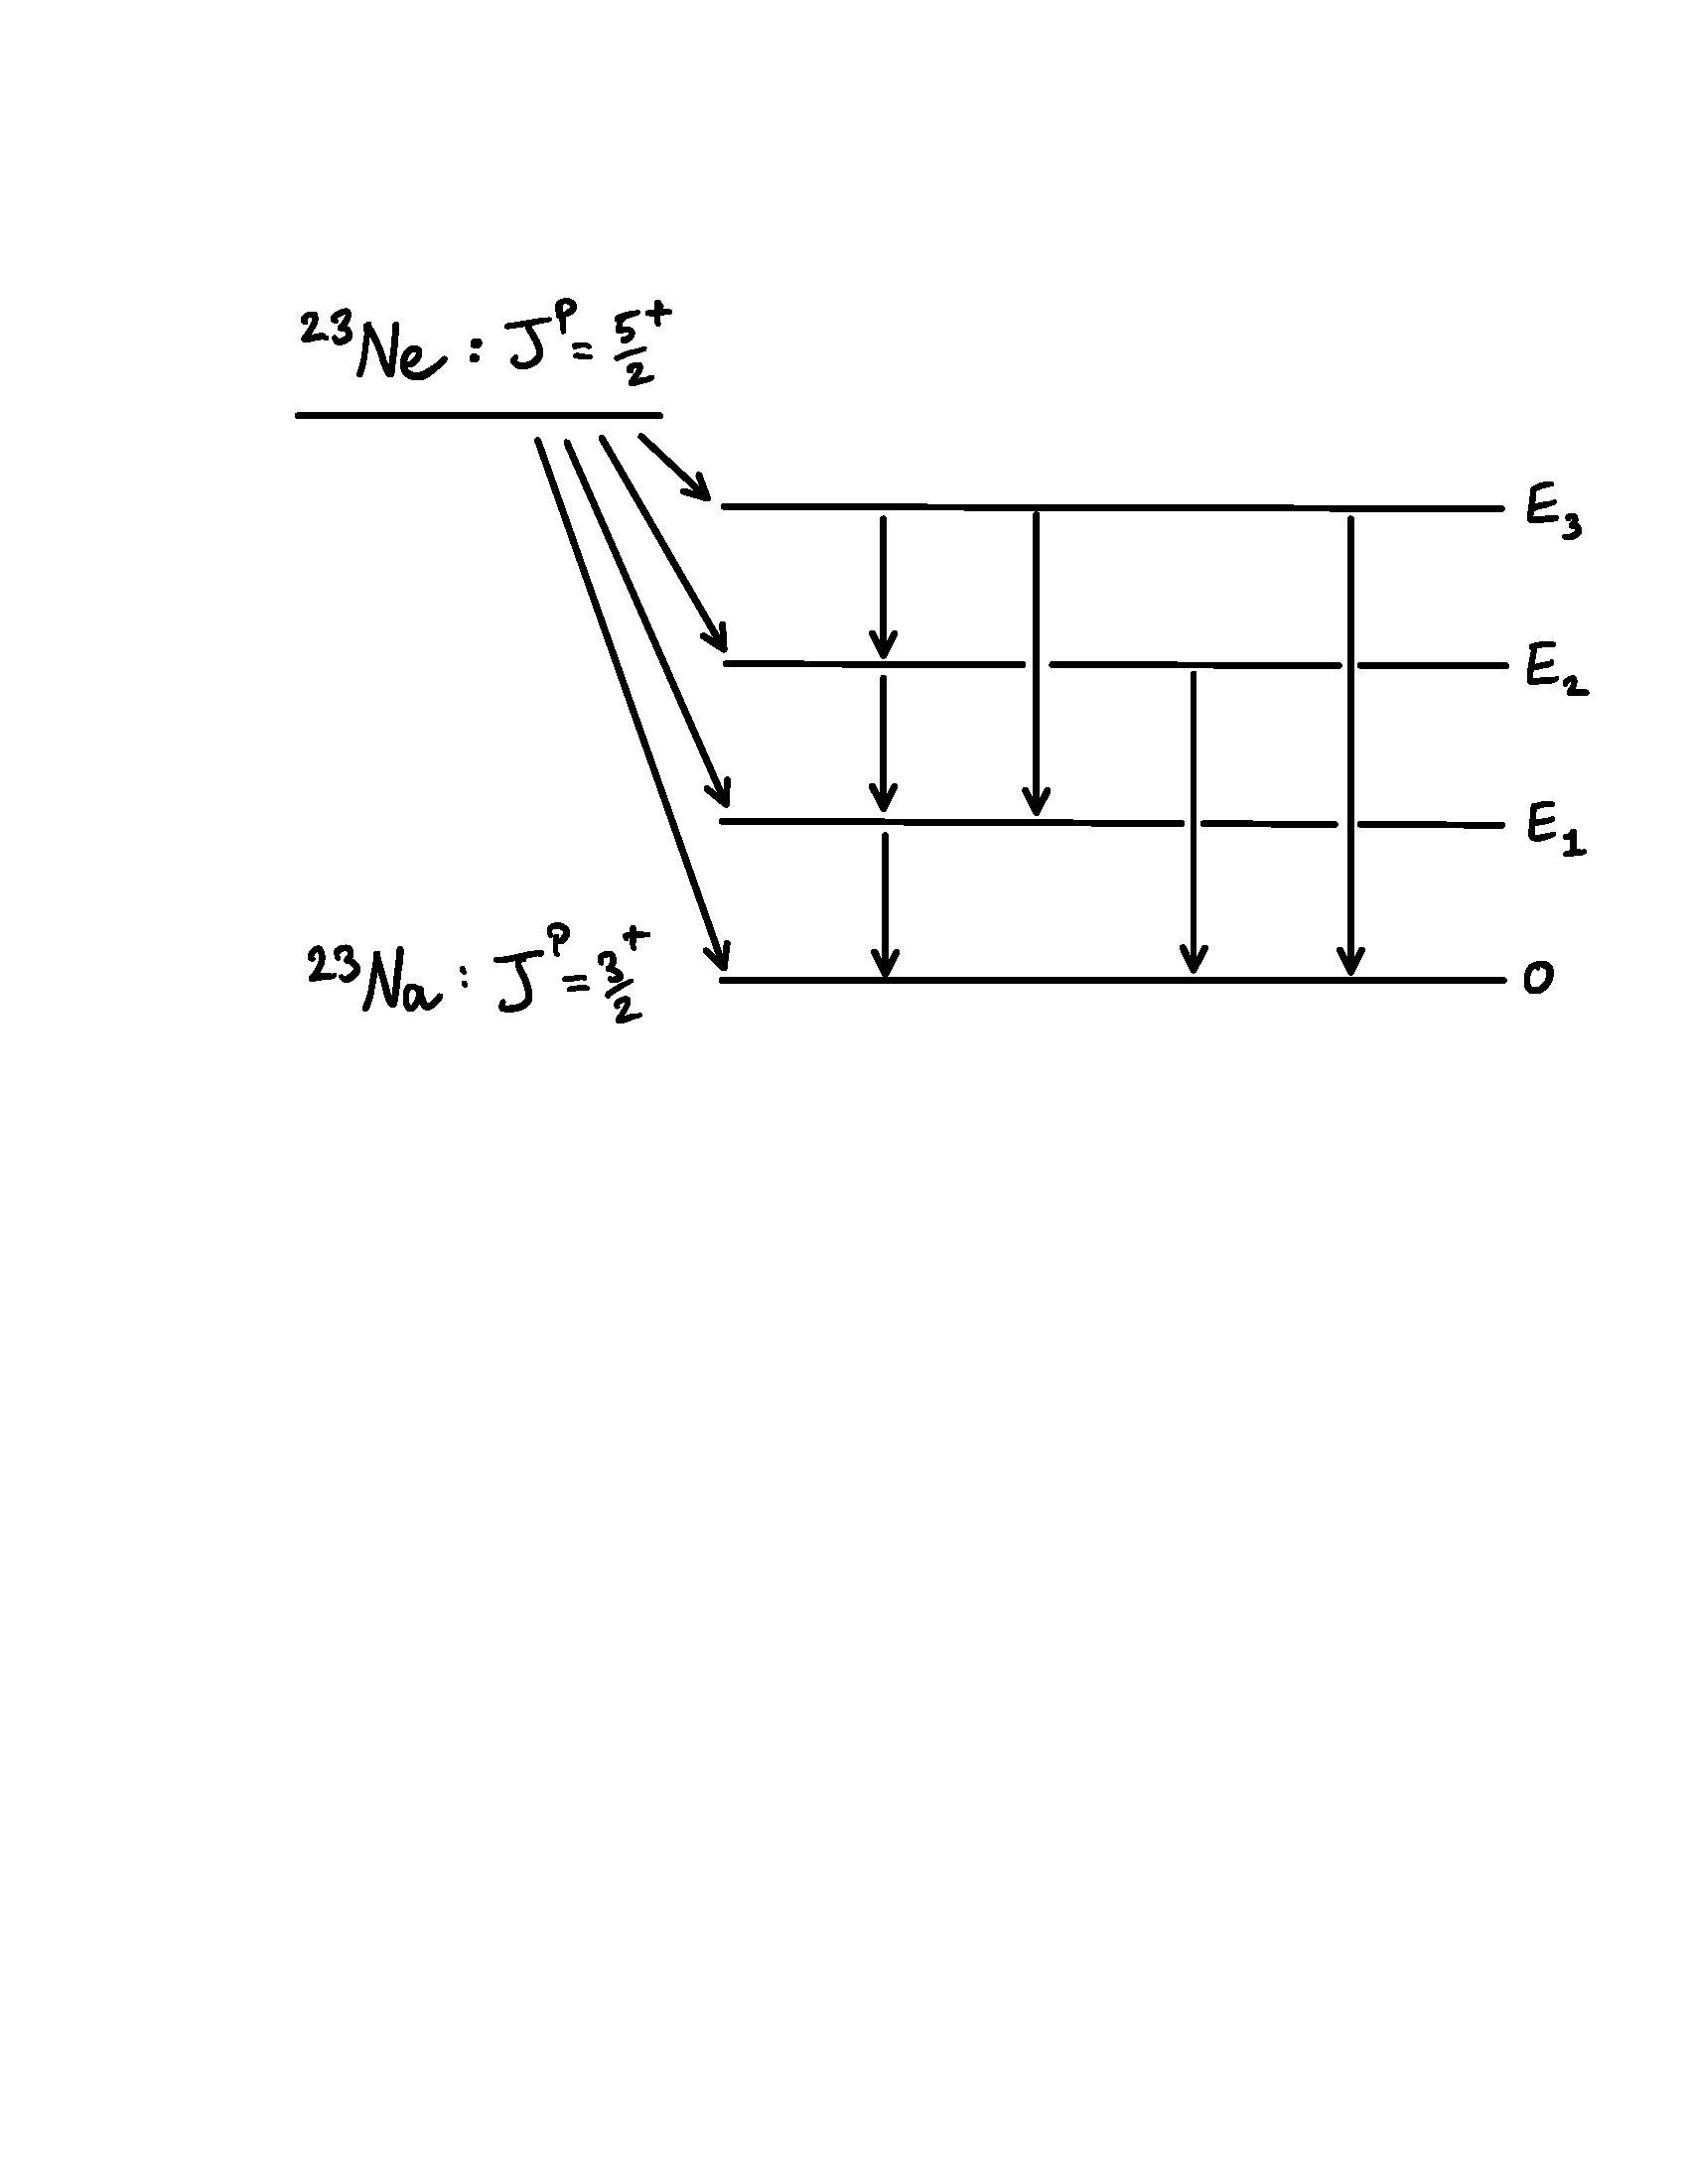
\includegraphics[width=0.65\textwidth]{Images/23Na_energy_levels_ipad.pdf}\end{center}

\ANS{

Any scheme can be inverted to produce a second scheme since $|E_i-E_j| = |E_j-E_i|$. There is only one fundamental four-level scheme that fits the data. We call its non-inverted and inverted variants `Scheme A' and `Scheme B'.  They look like this:


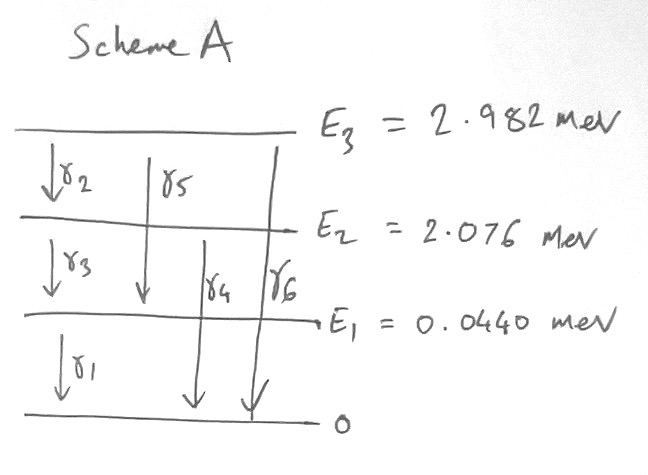
\includegraphics[width=0.7\textwidth]{Images/Scheme_A.jpeg}
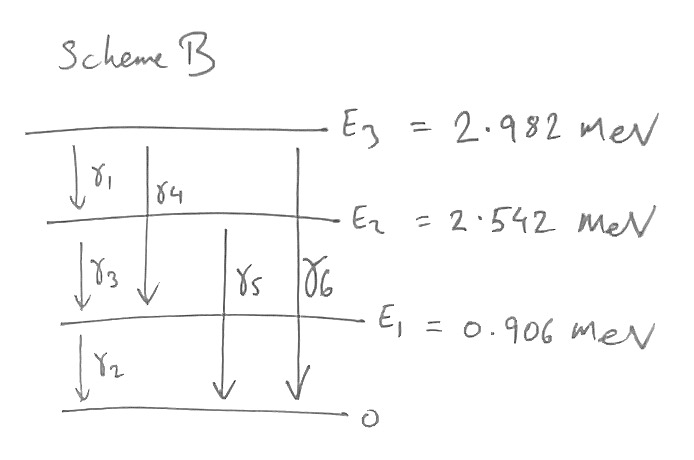
\includegraphics[width=0.7\textwidth]{Images/Scheme_B.jpeg}

}
\end{allparts}
%awk 'BEGIN{g=0;e1=0.440;e2=2.076;e3=2.982; print 1,e1-g, 2,e3-e2,3,e2-e1,   4,e2-g,   5,e3-e1,   6,e3-g;  print; b3=0.065/100; b2=1.10/100;b1=32/100; b0=1-b1-b2-b3; print b0,b1,b2,b3,":",b0+b1+b2+b3;          b32=0.04/100; b31=41.1/100; b30=1-b32-b31; b21=91.1/100; b20=1-b21;  print b30,b31,b32,":",b30+b31+b32 ;    print b21,b20,":",b21+b20;   b10=1;  r3=b3;  i32=r3*b32; i31=r3*b31; i30=r3*b30;    r2=b2+i32;    i21=r2*b21; i20=r2*b20;    r1=b1+i31+i21;      i10=r1*b10;    r0=b0+i30+i20+i10; print r0," should be 1";     i1=i10; i2=i32; i3=i21; i4=i20; i5=i31; i6=i30;      scale=3000000/0.78 ;  print scale*i1,scale*i2,scale*i3,scale*i4,scale*i5,scale*i6;  print;                  print scale*(i1+i4+i6),"    moo     ",scale*(i1-i3-i5),scale*(i3+i4-i2),scale*(i2+i5+i6); print;print;print;VV1=(i1-i3-i5);VV2=(i3+i4-i2);VV3=(i2+i5+i6);print (1-VV1-VV2-VV3),VV1,VV2,VV3 }'
%1 0.44 2 0.906 3 1.636 4 2.076 5 2.542 6 2.982
%
%0.66835 0.32 0.011 0.00065 : 1
%0.5886 0.411 0.0004 : 1
%0.911 0.089 : 1
%1  should be 1
%1.27034e+06 1 38543.2 3765.47 1027.5 1471.5
%
%1.27558e+06    moo      1.23077e+06 42307.7 2500
%
%
%
%0.66835 0.32 0.011 0.00065


\noindent
Observation of a large sample of  ${}^{23}\mathrm{Ne}$ undergoing complete decay reveals  that the numbers of emitted gamma rays having energies $\gamma_1,\gamma_2,\ldots,\gamma_6$ are (in that order) in the relative ratios $N_1:N_2:\ldots:N_6$ with $N_1=1.27\times 10^6$, $N_2=1.00$, $N_3=3.85\times 10^4$, $N_4=3.77\times10^3$, $N_5=1.03\times10^3$ and $N_6=1.47\times 10^3$.
\begin{allparts}
\part
Which energy-level scheme found in part (b) is the most probable given the gamma ray emission-ratio information just given?  Justify your choice.\marks{2}

\ANS{

Other things being equal, Ne would prefer to decay to Na states which are closer to its ground state than those which are more excited;  on the whole the greater energy drop makes the larger transitions more favourable. [1/2 mark]  The transition with energy $\gamma_1$ has the biggest intensity by far ($N_1\gg  N_i$ for all $i\ne1$).  Scheme B has $\gamma_1$ as a transition between levels 3 and 2, while Scheme A has this as a transition between level 1 and the ground state. Scheme B is impossible, therefore, as there should be at least as many gamma transitions OUT of any given unstable energy level as there are gamma transitions INTO that same level\footnote{Non-gamma (i.e.,~beta) transitions directly into the second Na level from Ne would account for the rest needed to balance the INs with the OUTs for level 2.} [1 mark] ... yet $N_3+N_5$ (which is proportional to transitions OUT of level 2 in Scheme B) does not equal or exceed $N_1$ (which is proportional to gamma transitions INTO state 2). Scheme A is therefore the correct one. [1/2 mark]

}

\part
For the most-probable scheme identified in (c) above, and denoting the branching ratios of ${}^{23}\mathrm{Ne}$ to the $0^\textrm{th}$, $1^\textrm{st}$, $2^\textrm{nd}$ and $3^\textrm{rd}$ excited states of ${}^{23}\mathrm{Na}$ by the symbols $\Gamma_0$, $\Gamma_1$, $\Gamma_2$ and $\Gamma_3$  respectively:
\begin{subparts}
\subpart
write down a simple equation relating $\Gamma_0$, $\Gamma_1$, $\Gamma_2$ and $\Gamma_3$; \marks{2}
\subpart
write down additional formulae relating $\Gamma_1$, $\Gamma_2$ and $\Gamma_3$ to the symbols $N_1,\ldots,N_6$ and $\Gamma_0$ so that you may: \marks{8}
\subpart
solve all the equations above simultaneously to determine the numerical values of $\Gamma_1$, $\Gamma_2$ and $\Gamma_3$ under the assumption that $\Gamma_0 =67$\%.\marks{2}
\end{subparts}
%\shorthint{You should avoid substituting numerical values into equations, even the value of $\Gamma_0$, until the end of any calculation.}%\marks{12}


\ANS{

The first part is simple. By definition:
$\Gamma_0+\Gamma_1+\Gamma_2+\Gamma_3=1$.

The second and third parts take more time:

The quantities $N_i$ specify \textbf{relative} intensities (or \textbf{relative} rates) but do not fix \textbf{absolute} ones.  Use this freedom, therefore, to work in an imaginary scenario in which the absolute rate of production of 23Ne is one nucleus per unit time.  In this scenario, the numerical values for the branching ratios $\Gamma_i$ are also the rates for the production (via beta decay) of the $i^\textrm{th}$ excited state.  Furthermore, denoting by $\rho_i$ the rate of production of $\gamma_i$, we will have $\rho_i = k N_i$ for some (unknown) constant $k$ which is independent of $i$.  With that notation we are in a position to write down an equation which expresses the idea that the number of decays INTO level 3 must be the same as the number of decays OUT OF level 3:
$$ \Gamma_3 = \rho_2+\rho_5+\rho_6.$$
Similarly, the equation which expresses the idea that the number of decays INTO level 2 must be the same as the number of decays OUT OF level 2 is:
$$ \Gamma_2 + \rho_2 = \rho_3+\rho_4$$
while that balancing inflows and outflows for level 1 is:
$$\Gamma_1+\rho_3+\rho_5 = \rho_1.$$
Finally the statement that `all the neon ends up in the ground state' is
$$\Gamma_0+\rho_1+\rho_4+\rho_6=1.$$

\noindent[Aside: adding the four equations above and then cancelling the expression  $\sum_{i=1}^6 \rho_i$ which appears on both sides  reproduces the first equation we wrote down: $$\Gamma_0+\Gamma_1+\Gamma_2+\Gamma_3=1.$$ 
We do not need to notice this fact, but it is a sensible consistency check!]


\noindent The vector of branching ratios
$[\Gamma_0,\Gamma_1 , \Gamma_2 , \Gamma_3]$ is therefore
\begin{align}
[\Gamma_0,\ \Gamma_1,\  \Gamma_2 ,\  \Gamma_3]
&=
[1-(\Gamma_1+\Gamma_2+\Gamma_3),
\Gamma_1 , \Gamma_2 , \Gamma_3]\nonumber
\\
&=
[ 1-(\rho_1+\rho_4+\rho_6)
,\ 
(\rho_1-\rho_3-\rho_5)
,\ 
(\rho_3+\rho_4-\rho_2)
,\ 
(\rho_2+\rho_5+\rho_6)
]\nonumber
\\
&=
[ 1 -(N_1+N_4+N_6)k
,\ 
(N_1-N_3-N_5)k
,\ 
(N_3+N_4-N_2)k
,\ 
(N_2+N_5+N_6)k
]\nonumber
%\\
%&=
%k[\frac 1 k - 1.27558\times %10^6,(N_1-N_3-N_5)
%,
%(N_3+N_4-N_2)
%,
%(N_2+N_5+N_6)].\nonumber
%\\
%&=
%k[\frac 1 k - 1.27558e+06, 1.23077\times10^6 , 42307.7 , 2500].\nonumber
.
\end{align}
In particular: $$\Gamma_0=1-(N_1+N_4+N_6)k$$ and so \begin{align}k= \frac{1-\Gamma_0}{N_1+N_4+N_6}.\label{eq:thingfork}\end{align}
\hide{which means that 
\begin{align}
[\Gamma_0,\Gamma_1 , \Gamma_2 , \Gamma_3]
&=
[\Gamma_0
,
\frac{N_1-N_3-N_5}{N_1+N_4+N_6}(1-\Gamma_0)
,
\frac{N_3+N_4-N_2}{N_1+N_4+N_6}(1-\Gamma_0)
,
\frac{N_2+N_5+N_6}{N_1+N_4+N_6}(1-\Gamma_0)
].\nonumber
\end{align}
}

\noindent The question gives values of $N_i$ from which we can compute that:
\begin{align}
N_1-N_3-N_5&\approx 1.23\times10^6
\\
N_3+N_4-N_2&\approx 42300 
\\
N_2+N_5+N_6&\approx 2501.
\end{align}
The question also tells us $\Gamma_0=0.67$ and so \eqref{eq:thingfork} implies:
\begin{align}
k
&=
\frac{1-0.67}{1.27\times 10^6+3.77\times10^3+1.47\times 10^3}\nonumber
\\
&=\frac{0.33}{1.275240\times 10^6}\nonumber
\\
&\approx 2.59\times 10^{-7}\nonumber
\end{align}
and hence putting the above together:
\begin{align}
[\Gamma_0,\Gamma_1 , \Gamma_2 , \Gamma_3]
&\approx
[0.67,
( 1.23\cdot 10^6)\cdot (2.59\cdot 10^{-7}), 42300 \cdot (2.59\cdot 10^{-7}), 2501\cdot (2.59\cdot 10^{-7})
]\nonumber
\\
&\approx
[0.670,
0.318, 0.0109, 0.00065]\nonumber
\\
&=
[67.0\%, 31.8\%, 1.09\%, 0.065\%]. \nonumber
\end{align}
This question is based on Fig 14 in  \url{http://dx.doi.org/10.1140/epja/i2018-12526-2} and was designed to give the branching ratios it reports.

\POSTMARKING{
An early draft this question asked the candidates to calculate the spins of the different Sodium levels in addition to what appeared in the final paper. However, that early draft was thought too hard and so the question was simplified to the one presented.  With hindsight the simplified question may have become  too simple as it  ended up with the highest fraction of 19/19 (i.e.~100\%-scoring) answers of any Part II exam question I have ever marked.  Many students found slightly tidier/shorter ways of doing the maths that got them to the final answer quicker than my answer above. Maybe they have access to simultaneous equation solving algorithms on their calculators? I don't mind if they do, as it's the physics that was being tested, not the maths. I am pleased, therefore, that so many students did get 100\% on this question because it means that it wasn't pitched too hard.
}
}


\end{allparts}
\hide{
The ground state of ${}^{23}\mathrm{Na}$ is known to have $J^P={\frac 3 2}^+$. Suppose that transitions $\gamma_2$ and $\gamma_4$ are known to be E2 (electric quadrupoles), while all the other transitions are M1/E2 (magnetic dipole or electric quadrupole).

\begin{allparts}
\part
What are the spins and parities of the excited states of ${}^{23}$Na which are produced in decays of ${}^{23}$Ne ?\marks{4}

\answer

At this point we have 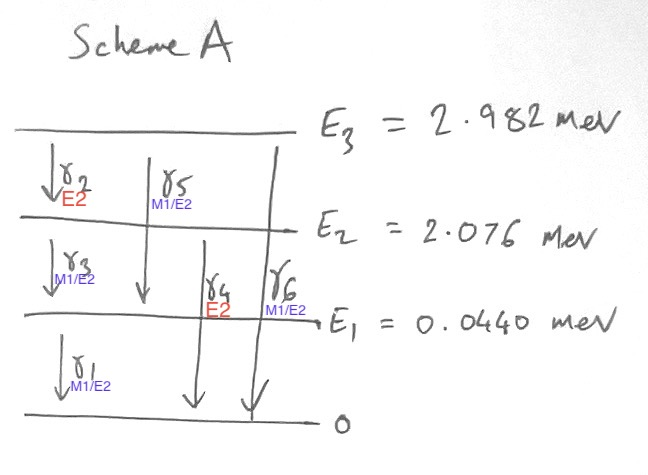
\includegraphics[width=0.7\textwidth]{Images/Scheme_A_with_poles.jpeg}

\begin{itemize}
\item
Neither E2 nor M1 induce a parity change, therefore all the excited states we are looking at have parity $P=+$ just like the ground state.
\item
The presence of an E2 transition ($\gamma_4$) from level-2 to ground together with the absence of an M1 for the same gap means that level-2 has a spin that is two units away from the ground state.  This fixes level-2 as $J^P={\frac 7 2}^+$
\item
The presence of an M1 transition between level-1 and EVERY OTHER STATE means that level-1 is at most one unit of spin away from every other level. But with other levels already at ${\frac 3 2}^+$ and ${\frac 7 2}^+$, that leaves only one possibility: level-1 has $J^P={\frac 5 2}^+$.
\item
The presence of an E2 transition ($\gamma_2$) from level-3 to level-2 together with the absence of an M1 for the same gap means that level-3 has a spin that is two units away from level-2.  This suggests level-3 is either  ${\frac 3 2}^+$ or ${\frac {11} 2}^+$.  The latter option is excluded by the M1 transition ($\gamma_5$) from level-3 to level-1.  Therefore level-3 is $J^P={\frac 3 2}^+$.
\end{itemize}
In summary, we have (as reproduced from Fig 14 of \url{http://dx.doi.org/10.1140/epja/i2018-12526-2} )

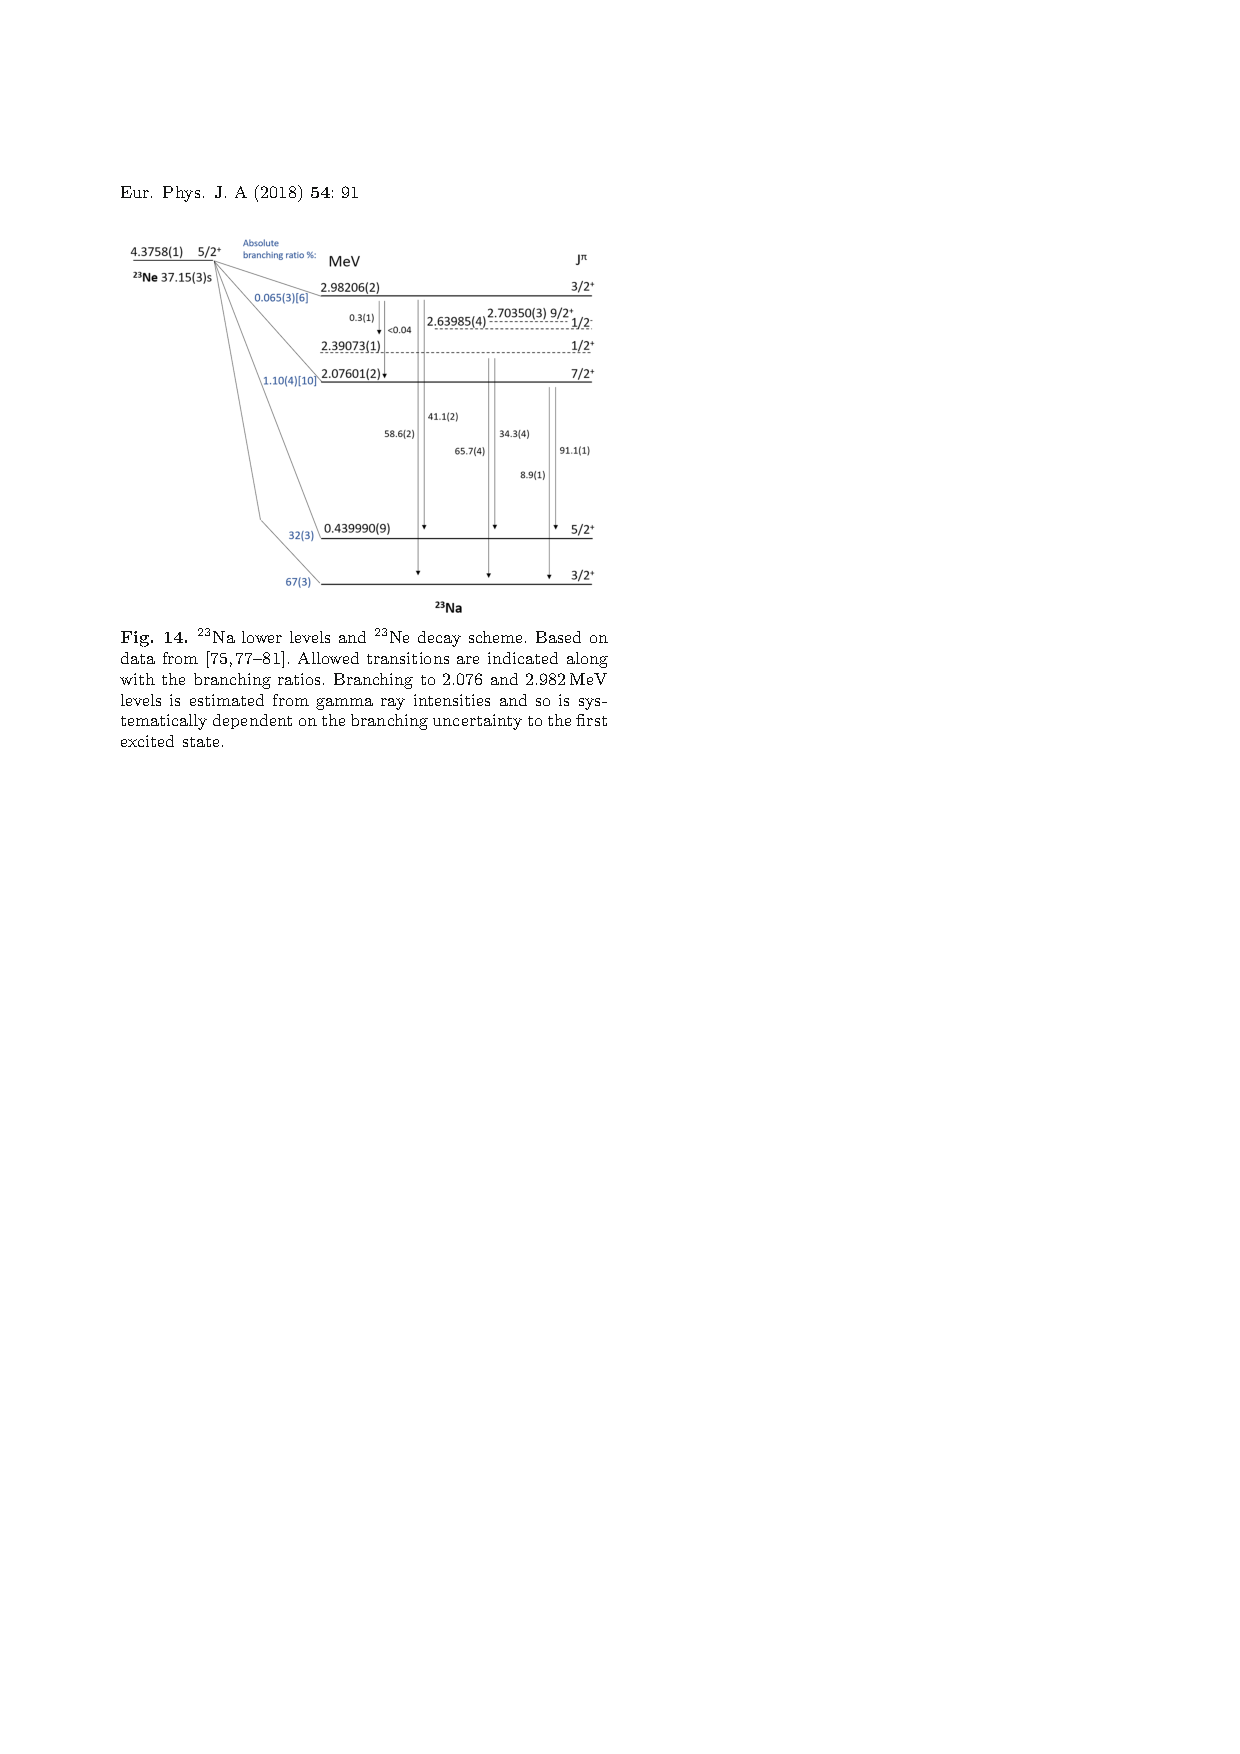
\includegraphics[width=0.8\textwidth]{Images/23Na_spectrum_from_paper.pdf}

\endanswer

\end{allparts}
}
%\vspace{3cm}

%%%%%%%%%%%%%%%%%%%%%%%%%%%%%%%%%%%%%%%%%%%%%%%%%%%%%%%%%%%%%%%%%%%

\clearpage
\question

\noindent 
\startpart

%\noindent
%{}
\begin{allparts}
\part
Explain how the hadron wavefunction
$$\psi_\mathrm{hadron} = \psi_\mathrm{space}\psi_\mathrm{spin}\psi_\mathrm{flavour}\psi_\mathrm{colour}$$
leads to the prediction of an octet of spin-$\frac 1 2$ states and a decuplet of spin-$\frac 3 2$ states for the
lowest-mass baryons formed from up, down and strange quarks.\marks{6}
\ANS{BOOKWORK: Standard from the lecture notes.}
\part
Briefly explain the origin of the baryon mass formula
$$M_{qqq} = m_1 +m_2 +m_3 +A'\left[
\frac{\vec S_1 \cdot \vec S_2}{m_1 m_2}
+
\frac{\vec S_2 \cdot \vec S_3}{m_2 m_3}
+
\frac{\vec S_3 \cdot \vec S_1}{m_3 m_1}
\right],$$
where $A'$ is a constant.\marks{2}
\ANS{BOOKWORK: Standard from the lecture notes.}
\part
Derive the specific form  the above mass formula takes for the  case of a spin-$\frac 1 2$ baryon composed of one up and two strange quarks. Repeat this exercise to determine how the mass of a spin-$\frac 3 2$  bound state with the same quark content depends on the same quantities.  \shorthint{In both cases show your working and leave each answer in terms of $m_u$, $m_s$ and $A'$ only.}  
\marks{8}

\ANS{

The answer is:

\begin{align*}
M_{uss} & =
\begin{cases}m_u + 2m_s + A'\left[
\frac 1 {4 m_s^2} - \frac 1 {m_u m_s} \right]
& \text{for $J^P={\frac1 2}^+$ and}
\\
 m_u + 2m_s + A'\left[
\frac 1 {4 m_s^2} + \frac 1 {2m_u m_s}\right] & \text{for $J^P={\frac3 2}^+$.}
\end{cases}
\end{align*}

The derivation follows.

There are two like-flavour quarks ($ss$) and one other-flavour quark ($u$). Label the three quarks `1', `2' and `$u$' with the numbers distinguishing the two $s$-quarks.

The `hard' part of this calculation is finding 
$$
\frac{\vec S_1 \cdot \vec S_2}{m_1 m_2}
+
\frac{\vec S_2 \cdot \vec S_3}{m_2 m_3}
+
\frac{\vec S_3 \cdot \vec S_1}{m_3 m_1}.
$$
Fortunately we do not need to compute each of  $\vec S_1\cdot \vec S_2$, $\vec S_1\cdot \vec S_3$ and $\vec S_2\cdot \vec S_3$ separately.  Because:
\begin{align}
\frac{\vec S_1 \cdot \vec S_2}{m_1 m_2}
+
\frac{\vec S_2 \cdot \vec S_3}{m_2 m_3}
+
\frac{\vec S_3 \cdot \vec S_1}{m_3 m_1}
&=
\frac{\vec S_1 \cdot \vec S_2}{m_s^2}
+
\frac{\vec S_2 \cdot \vec S_u}{m_s m_u}
+
\frac{\vec S_u \cdot \vec S_1}{m_u m_s}\nonumber
\\
&=
\frac{\vec S_1 \cdot \vec S_2}{m_s^2}
+
\frac{\left(\vec S_1+\vec S_2\right) \cdot \vec S_u}{m_u m_s}\label{eq:forsubback}
\end{align}
we only need to compute $\vec S_1 \cdot \vec S_2$ and $\left(\vec S_1+\vec S_2\right) \cdot \vec S_u$.

We recall from the earlier discussion of hadron wavefunctions that we need to consider wave functions for which the FLAVOUR*SPIN parts are symmetric overall. It is not possible to have wave functions which are flavour-odd with respect to the two like-flavour $s$-quarks, and so the resulting flavour-even wavefunction needs to be combined with one which is has an even (i.e. triplet) spin wave function (such as  $\phi^{\text{spin}}_{1 2}=\frac 1 {\sqrt 2} ( \uparrow \downarrow + \downarrow \uparrow)$ or  $\uparrow\uparrow$ or $\downarrow\downarrow$) for quarks `1' and `2'.  I.e. $S_{12}=1$. The difference between the $J=\frac 1 2$ and $J=\frac 3 2$ states will thus be created by  the third quark (the $u$) adding its own $S_3=S_u=\frac 1 2$ either destructively or constructively to the mix.

Considering just the two like quarks we have:
\begin{align}
\vec S_{12}^2 
&= 
\vec S_1^2 +
\vec S_2^2 +
2\vec S_1\cdot \vec S_2
\end{align}
which gives:
\begin{align}
\vec S_1\cdot \vec S_2
&=
\frac 1 2 \left(
\vec S_{12}^2 
-
\vec S_1^2 -
\vec S_2^2 \nonumber
\right)\\
&=
\frac 1 2
\left(
S_{12}(S_{12}+1)
-
S_{1}(S_{1}+1)
-
S_{2}(S_{2}+1)\nonumber
\right)\\
&=
\frac 1 2
\left(
1
\times(1+1)
-
{\frac 1 2}\times({\frac 1 2}+1)
-
{\frac 1 2}\times({\frac 1 2}+1)
\right)\nonumber
\\
&= \frac 1 4 \label{eq:quarter}
\end{align}
which is one of the two main things we set out to find.

Using the above we can then move on and find $\left( \vec S_1+\vec S_2\right) \cdot \vec S_u$ via
\begin{align*}
\vec S^2 
&= 
\vec S_1^2 +
\vec S_2^2 +
\vec S_u^2 +
2 \left( \vec S_1+\vec S_2\right) \cdot \vec S_u 
+ 2\vec S_1\cdot \vec S_2
\end{align*}
which tells us that
\begin{align*}
\left( \vec S_1+\vec S_2\right) \cdot \vec S_u 
&=
\frac 1 2
\left(
\vec S^2 -\left(\vec S_1^2 +
\vec S_2^2 +
\vec S_u^2\right)
-2 \vec S_1\cdot \vec S_2
\right)
\\
&=
\frac 1 2 \left(
J(J+1) - 3\times\left(\frac 1 2 \times \left(\frac 1 2 + 1\right)\right) -
2\times \frac 1 4
\right)
\\
&=
\frac 1 2 J (J+1) - \frac {11}8
\\
&=\begin{cases}
-1 & \text{when $J=\frac 1 2$}\\
+\frac 1 2 & \text{when $J=\frac 3 2$.}\\
\end{cases}
\end{align*}
We can now substitute the values we have just computed for $\vec S_1 \cdot \vec S_2$ and $\left(\vec S_1+\vec S_2\right) \cdot \vec S_3$ back into equation (\ref{eq:forsubback}) and put it together with the (trivial) mass terms to get the baryon mass formulae  given at the start of this answer.
}
\part
The $\Xi^0$ ($J^P={\frac1 2}^+$) and $\Xi^{*0}$ ($J^P={\frac3 2}^+$) baryons are bound states of $uss$ quarks.  Using your formulae from part (c), calculate numerical values for mass predictions for the $\Xi^0$ and $\Xi^{*0}$. \shorthint{The quark masses may be taken to be $m_u = 362~\mathrm{MeV}$ and $m_s = 537~\mathrm{MeV}$.  $A' = 0.026~\mathrm{GeV}^3$.}\marks{1}

\part
The experimentally measured values of the masses are $M(\Xi^0)=1314.86\pm0.20$~MeV and $M(\Xi^{*0})=1531.79\pm0.34$~MeV.  What level of agreement between predicted and measured masses might one reasonably expect the baryon mass formula to provide, and is the level of agreement you saw in (d) better or worse than this?\marks{2}
%
%\noindent

\ANS{

THIS IS THE ANSWER TO (d) and (e) TOGETHER

To three significant figures\footnote{Aside: these answers are probably right to three sig figs (even though the quantity $A'$ is only given to two significant figures) since $A'$ controls the difference (about 200 MeV) between the two values for $M_{uss}$ -- while the absolute value is in the region of 1000 MeV and is controlled by $m_u$ and $m_s$ which were given to higher precision. The prediction (looking at just the maths and error propagation, but ignoring systematic uncertainties) ought therefore to be good to $\pm10$~MeV.} the baryon mass formula just derived yields:  $M(\Xi^0)\sim 1320$~MeV and $M(\Xi^{*0})\sim 1530$~MeV.  These  values are compatible with the experimental results to within the computed values' stated precisions. If anything, the surprise here is that the computed values are so close.  The model is very simple (totally ignoring gluons, sea quarks, and  myriad other non-perturbative effects).  Not only that, but quark masses themselves are very much measurement-method-dependent (since colour confinement prevents quarks from being isolated), so one does not have much confidence that the supplied quark masses are even meaningful for this problem. Most baryon mass predictions are therefore not this good, and this level of agreement is therefore much better than we have a right to expect.
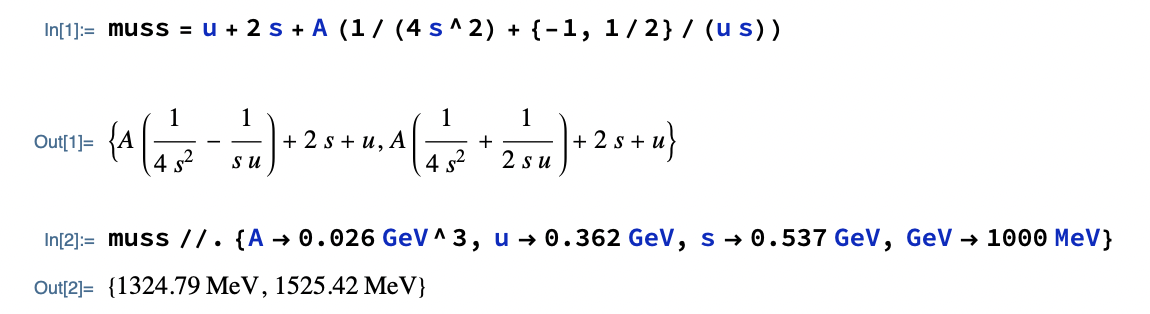
\includegraphics[width=0.7\textwidth]{Images/baryon_mass_calc.png}

}

\end{allparts}

%\begin{allparts}
%\part
%\end{allparts}

%%%%%%%%%%%%%%%%%%%%%%%%%%%%%%%%%%%%%%%%%%%%%%%%%%%%%%%%%%%%%%%%%%%

\clearpage
\question

\noindent 
\startpart

\noindent
Some parts of this question expect you to extract information from a  set of tables reproduced from the latest edition of `The Review of Particle Physics'.
These tables (which can be found after the statement of the question) may include both information which is irrelevant to you, and terms or symbols which are not fully explained. The question is therefore testing your ability to extract information from unfamiliar  sources regularly used in particle physics research.
\begin{allparts}
\part
Explain why the positively charged pion's decay mode to $\mu^+\nu_\mu$ dominates over its decay to $e^+\nu_e$.\marks{3}

\ANS{
BOOKWORK: description of parity violation, angular momentum conservation, scalar nature of pion, neutrinos all left handed, etc.

\POSTMARKING{
I expected this to be the easiest three marks on the paper as it is a question that has been asked in many previous years (both in tripos and in the examples sheets) and generally (historically) has formed the main way of illustrating in lectures that the parity violation of the weak interaction has actual important consequences. I have lectured this course myself (a long time ago) and if I were to do so again I cannot imagine how I could introduce the weak interaction without somehow making a big thing of this material. However, those remarks aside, this year this question (6)(a) was arguably the worst answered question on the paper. Not only that, the most common answer which was offered by candidates was: `The muon is heavier than the electron, so there is greater phase space for the muon decay and so decay to muons happens more frequently than decays to electrons'. Alas, this answer shows a complete misunderstanding of phase space! [Because the muon is heavier it should have has LESS phase space in the final state than the electron, not MORE!]  So, in short, fewer than one in ten students could point out any link to parity at all, and nearly everyone else wrote something that showed they had systematically misunderstood (or reversed in their minds) the link between the size of phase space and the mass of a particle in the final state!  I don't know what the cause of this misunderstanding in the student body this year was, but it appears to have affected large numbers of them. I have not seen it in previous years.
}
}

\part
Looking at the decay modes of the $\pi^0$, suggest possible reasons for the difference between the branching fractions stated for the $e^+e^+e^-e^-$ and  $e^+e^-$ final states.\marks{4}

\ANS{
This is a tough question as the (strong) preference for the four-electron final state over the two-electron final state will be DOUBLY counter-intuitive to the students who have been brought up (1) vertex counting, and (2) looking at phase space.  [There are more vertices in the Feynman diagram for $\pi^0\rightarrow e^+e^+e^-e^-$  than for $\pi^0\rightarrow e^+e^+$, and the final state with four electrons is heavier than that with two!]  I am not looking for any specific or correct answer to this question [hence `suggest' rather than `state'/`explain']. Rather I am looking to see candidate making sensible statements which make clear that they are mentally processing (or even can see) the challenge faced by the discrepancy seen here.     E.g.,~there could be some marks for a candidate observing that the preference goes against a `simple' analysis for the two reasons already mentioned and so must be related to some other constraints/principles.  It is conceivable that some candidates will look at the decay table and note that $\pi^0\rightarrow \gamma\gamma$  dominates over all other decay modes by a long way. Though they may not know that this is due to $C$-parity ($C$-parity is not in the Part-II course lectures, but does come up in passing in Prob Sheet 2, Q13a) they may at least report that WHATEVER it is that leads to the favouring of $\gamma\gamma$ final states could lead to bleed-through into $\gamma e^+e^-$ and from there into $ e^+e^+e^-e^-$ as a result of off-shell photons going to $e^+e^-$. They might even note that this would account for the approximately equal spacing (in log space) of the branching ratios for those three modes. Perhaps candidates will have ideas that are very different from those I've suggested here. So long as they are intelligent statements derived from things they were learning about in the course, and are accurately applied, they will be rewarded, even if they don't ultimately explain the preference for four electrons. 

\POSTMARKING{
As mentioned above, I was not looking here for a `right' answer but just for some statements showing that candidates had learned that diagrams which need more QED vertices are (other things being equal) suppressed by powers of ~1/137 (ish) per vertex relative to diagrams with fewer, and that (therefore) there must be something `wrong' with the simplest/naivest  $\pi^0\rightarrow \gamma \rightarrow e^+e^+$ diagram as otherwise it would actually happen MORE easily than $\pi^0\rightarrow e^+e^+e^-e^-$. [The table tells us the rates are the other way around.]  Some candidates did get full marks for arguments they may have remembered from lectures that the difference between the pion spin (0) and the photon spin (1) prevented a single photon decay, thus forcing more complex diagrams for $\pi^0\rightarrow e^+e^+$, and then went (and were rewarded for) remarking on differences between propagators in those diagrams, and phase space issues. Others got nearly full marks for remaking on some other need for a complex diagram for the two electron final state. All good.  But a large fraction of candidates didn't do this and said things that didn't make sense ... e.g.~quite a few drew a complex four-vertex diagram for $\pi^0\rightarrow e^+e^+e^-e^-$ and a simple two-vertex diagram for  $\pi^0\rightarrow \gamma \rightarrow e^+e^+$  and then said that the extra vertices in their complex diagram would ENHANCE (!!) its cross section with respect to the paucity of vertices in the simpler diagram.  This may even have been a majority of the cohort.  This backwards arguing appears to show that almost the majority of candidates thought QED vertices make cross sections bigger rather than smaller!  As a result, the marks scored for this part were relatively low (often not more than 2 out of 4). Despite the poor mark average,  I don't feel the question was illegitimate: I believe that students on this course *should* have taken away from the course the message that (other things being equal) complex diagrams with more QED vertices are usually suppressed w.r.t.~simpler diagrams with fewer QED vertices (that is after all the entire basis of Feynman Diagrams and perturbative QED!) and so they should not find themselves in the position (as many did) of losing marks on account of having argued the reverse.
}
}

\part
Draw the lowest order Feynman diagrams for the processes (i) $\pi^0 \rightarrow \pi^+ e^- \bar \nu_e$ and (ii) $\pi^+ \rightarrow e^+ \nu_e \pi^0$. Why do the tables list a branching ratio for only one of these two processes?  What branching ratio is reported for it?  What physical reasons might lead to it being that big or that small?
\marks{5}

\ANS{
50\% of the marks are for just drawing valid Feynman diagrams containing a single $W$ connected to the right things (with no gluons or photons hanging around).  
Then they need to point out that the mass of the $\pi^+$ is bigger than that of the $\pi^0$ and so the $\pi^0$ cannot have decays involving $\pi^+$ on kinematic grounds.  The branching ratio for $\pi^+ \rightarrow e^+ \nu_e \pi^0$ is very small ($1.03\times 10^{-8}$).  An important point affecting the smallness of this branching ratio is that the $\pi^+$ and $\pi^-$ mass difference is itself very very small (only 4.5 MeV, relative to 140 MeV for the mass of the $\pi^+$ itself).  This means that there is already a factor of 30 (i.e.~140/4.5) more phase space for decays without a pion in the final state than for those with one. On top of that, there are extra vertices to throw into the calculation to generate the pion.  

}
\part
%Why is no decay mode table given for the $\pi^-$ ? 
Make a prediction for the $\pi^-$ branching fraction into (i) $\mu^-\bar\nu_\mu \gamma$ and (ii) $e^-\nu_e e^- e^+$.
\marks{2}

\ANS{
%The $\pi^-$ decay modes table is not given as decay modes can be inferred from the supplied $\pi^+$ table after $CP$-conjugating each row.  [1 mark] This is valid ias $CP$-violation is not important for pions. [1 marks]

Part (i) here is almost a dummy question whose purpose is not to check the answer ($(2.00\pm0.25)\times 10^{-4}$) but to make it clear that the question setter will put bars on neutrinos when required.  It is necessary to flag that willingness up here so that the part (ii) can be validly asked/answered.

The answer to part (ii) is \textbf{zero} because the CP conjugation of 
$e^-\nu_e e^- e^+$ is $e^+\bar\nu_e e^+ e^-$ and there is no such line in the PDG's $\pi+$ decay table. The table only has a line for $e^+\nu_e e^+ e^-$.  The suggested mode violates lepton number so the branching ratio is zero.


\POSTMARKING{
A few candidates noticed the (deliberate) letpon number non-conservation in part (ii) and instead of accepting it and writing B=0 they made a statement that they thought this was a typo (which it was not), then mentioned this overtly, then `corrected' the typo, and then wrote down the appropriate non-zero B from the PDG table.  I gave these candidates full marks (just like the candidates who wrote down the intended answer of B=0) as they were demonstrating the same skill of paying attention to particles-vs-antiparticles.  Candidates who, however, did not notice the lack of a bar and wrote down a non-zero B with no explanation lost the mark for (ii) as intended.  Roughly 80\% of students did not look at the bars.  A small number of students acted as if perhaps they thought there was a typo, though they did not explicitly say so. These students, in effect, answered a question I had not set (which they could be said to have set themselves) and which they answered correctly. To those students I gave a half mark if: (i) what they wrote was correct in itself, and (ii) if it included both sets of decay products correctly conjugated with respect to each other so that I could tell that they were indeed taking care to test for lepton flavour on the neutrino.  This was only 1/2 a mark (not a full mark) because those students were neither answering the question I had set, nor were unambiguously declaring that they were attempting to make an  correction (valid or otherwise) to the question on the paper.
}
}

\part
Suppose that a $\Xi^0$ baryon is produced in a vacuum at the centre of an infinitely large box at time $t_0=0$. 
What are the most probable contents of the box if inspected at a later time $t_1=10^{-12}$~s?  Describe the two main routes or `histories' through which the contents of the box might be expected to evolve over time.  Cover the period from $t_0$ until the contents of the box reach steady state, making clear on what timescales different events might be expected to happen.  How probable are the two end states you have considered? \marks{5}

\ANS{

This question asks the candidates to look at all the decay tables and plot a route through for the decay of the $\Xi^0$.  They should see the following:
\begin{itemize}
\item
The lifetime of the $\Xi^0$ is $\tau_\Xi=2.9\times 10^{-10}$~s, so very little can be expected to have happened on time scales much shorter than that (i.e.~by the time $t_1$ mentioned in the question the box will still contain just an undecayed $\Xi^0$).  Around 80\% of candidates got this first part right, but around 10\% said the most likely content at $t=t_0$ was a $\Lambda^0 \pi^0$.
\item
That by/around  $\tau_\Xi$ the $\Xi^0$ stands a good chance of having decayed, and if it has decayed, the vast majority of decays are to $\Lambda \pi^0$.
\item
However, the lifetime of the $\pi^0$ is $\tau_{\pi_0}=8\times 10^{-17}$~s which is much shorter than $\tau_\Xi$. Therefore, when the $\Xi$ decay eventually takes place it will (for all practical purposes) look like a decay to $\Lambda \gamma \gamma$ -- one has only a vanishing chance of being there at the right time to see both a $\Lambda$ and a not-yet-decayed $\pi_0$.
\item
The $\Lambda$ has a similar lifetime to the $\Xi$, so on a similar timescale to the $\Lambda$ being created it is likely to be replaced (with probability $\sim64$\%) by $p\pi^-$ or (with probability $\sim35$\%) by a $n\pi^0$ which will `instantly' become $n\gamma\gamma$.
\item
The lifetime of the $\pi^-$ is, however, longer than those we've seen before, $\tau_{\pi^-}=10^{-8}$~s (on account of helicity suppression) so the disappearance of the $\pi^-$ will take place over a time of order $\tau_{\pi^-}$.
\item By around $t=10^{-7}$~s all the $\pi^-$ will have died away and so we will either find the box containing $p\mu\bar\nu_\mu\gamma\gamma$ (with probability $\sim64$\%) or $n\gamma\gamma\gamma\gamma$ (with probability $\sim35$\%).
\item
At this point muon decay ($\mu^-\rightarrow \nu_\mu \bar\nu_e e^-$) could  be mentioned -- but the marker will not penalise persons who treat  muons as `stable' since no muon decay data has been provided.
\item
Things will stay much like that until the neutrons begin to decay, which should be complete when $t\gg 880$~s (the lifetime of the neutron).
\item
The final state is therefore $p\mu\bar\nu_\mu\gamma\gamma$ (with probability $\sim64$\%) or $p e^-\bar\nu_e\gamma\gamma\gamma\gamma$ (with probability $\sim35$\%).
\end{itemize}
One could award about half a mark per bullet point above.

\POSTMARKING{Although any question has a large spread in marks, this part (e) of question 6 was mostly very well answered -- at least by the candidates who had managed their time well and were not out of time at this point. People found many different ways of describing their answer, so there was lots of flexibilty from the marker in terms of what was deemed a valid format. However most people concluded with some kind of diagram like the one given below, and if they did it would have got them 100\%. Whether or not a given candidate included a diagram, \textit{roughly} a half a mark was awarded for each pink-highlighted `detail' on my diagram below, however it was communicated. The biggest source of marks lost (but those not under time pressure) was neglecting to consider neutron decay.  About 5\% of candidates lost marks by ignoring the instruction to report on histories up to the point in time at which a `steady state' had been reached. Such people tried to write complex histories for times between $t=0$ and $t=t_1$ only. %Most people assumed that the muon is stable (which it is not) as no muon data-table was given. I felt this was a reasonable thing for them to have done as the question was about data extraction, so I allowed people to treat the muon as stable or to treat it as unstable, whichever they preferred, for equal credit.

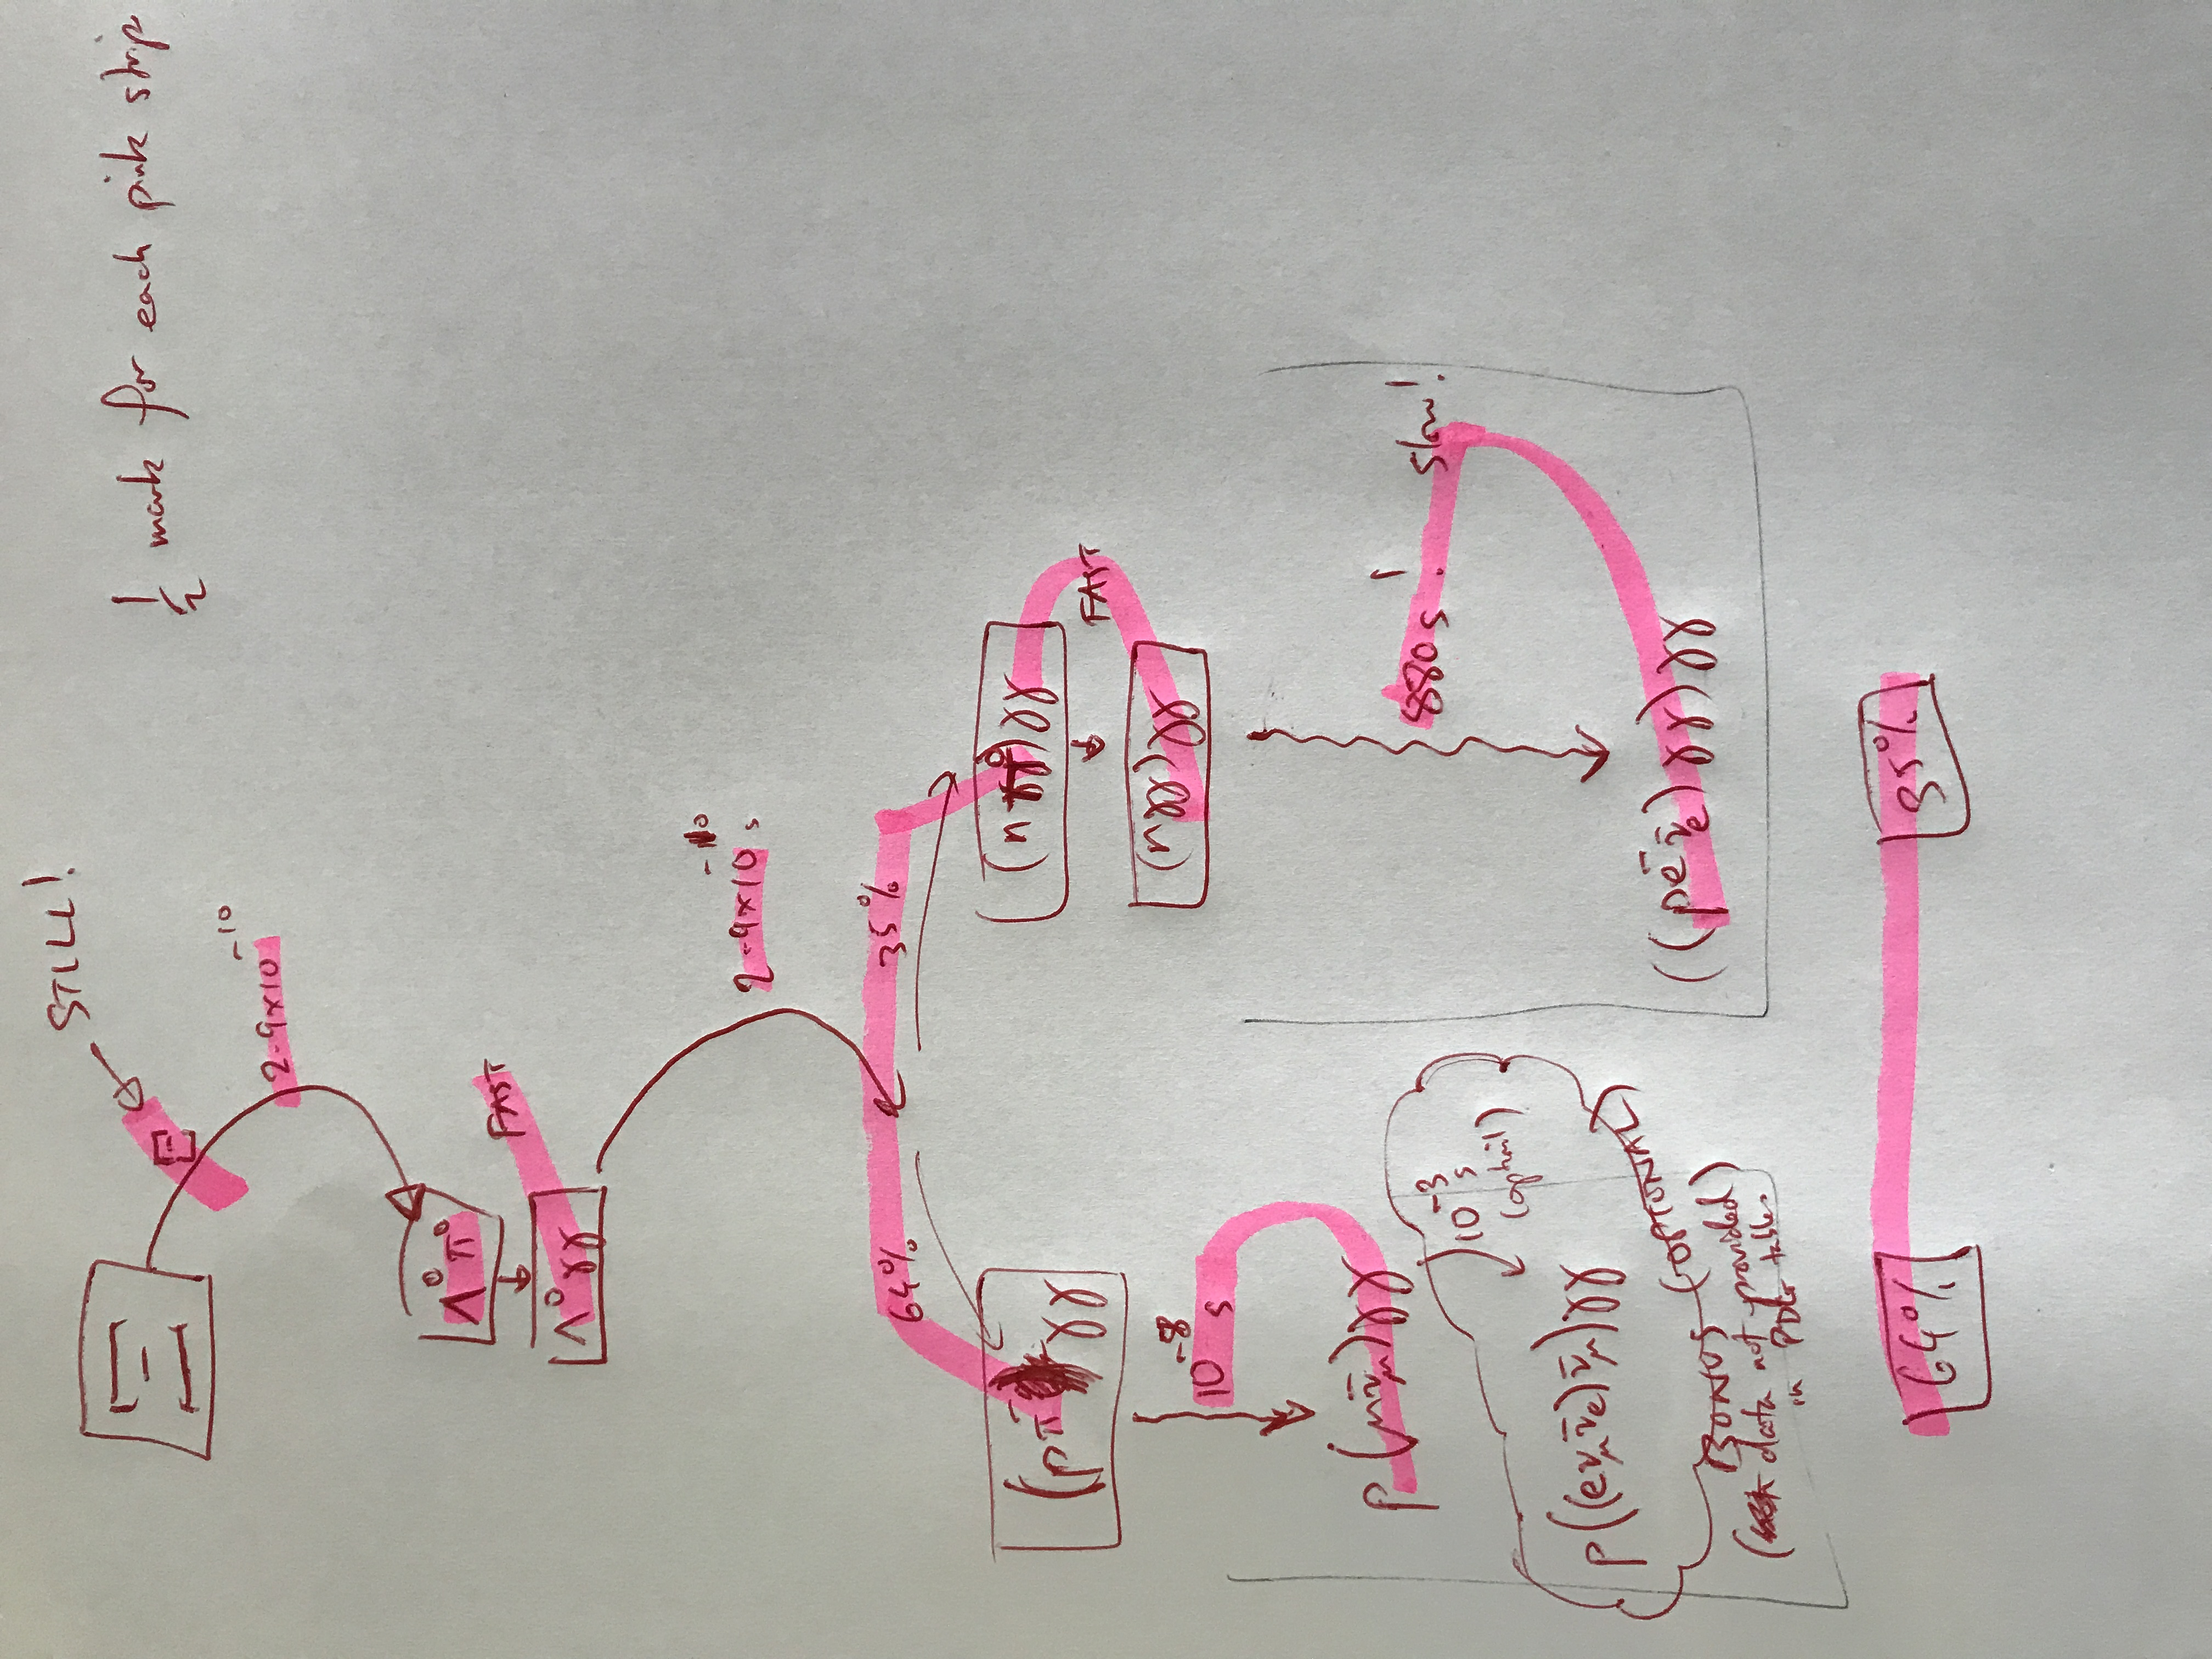
\includegraphics[width=1.0\textwidth,angle=-90]{Images/pinks.jpg}
}
}
\end{allparts}

%\begin{allparts}
%\end{allparts}

%\begin{allparts}
%\end{allparts}

%\begin{allparts}
%\end{allparts}

%\begin{allparts}
%\end{allparts}

%\begin{allparts}
%\end{allparts}

%\begin{allparts}
%\end{allparts}

%\begin{allparts}
%\end{allparts}

%\begin{allparts}
%\end{allparts}

\begin{center}
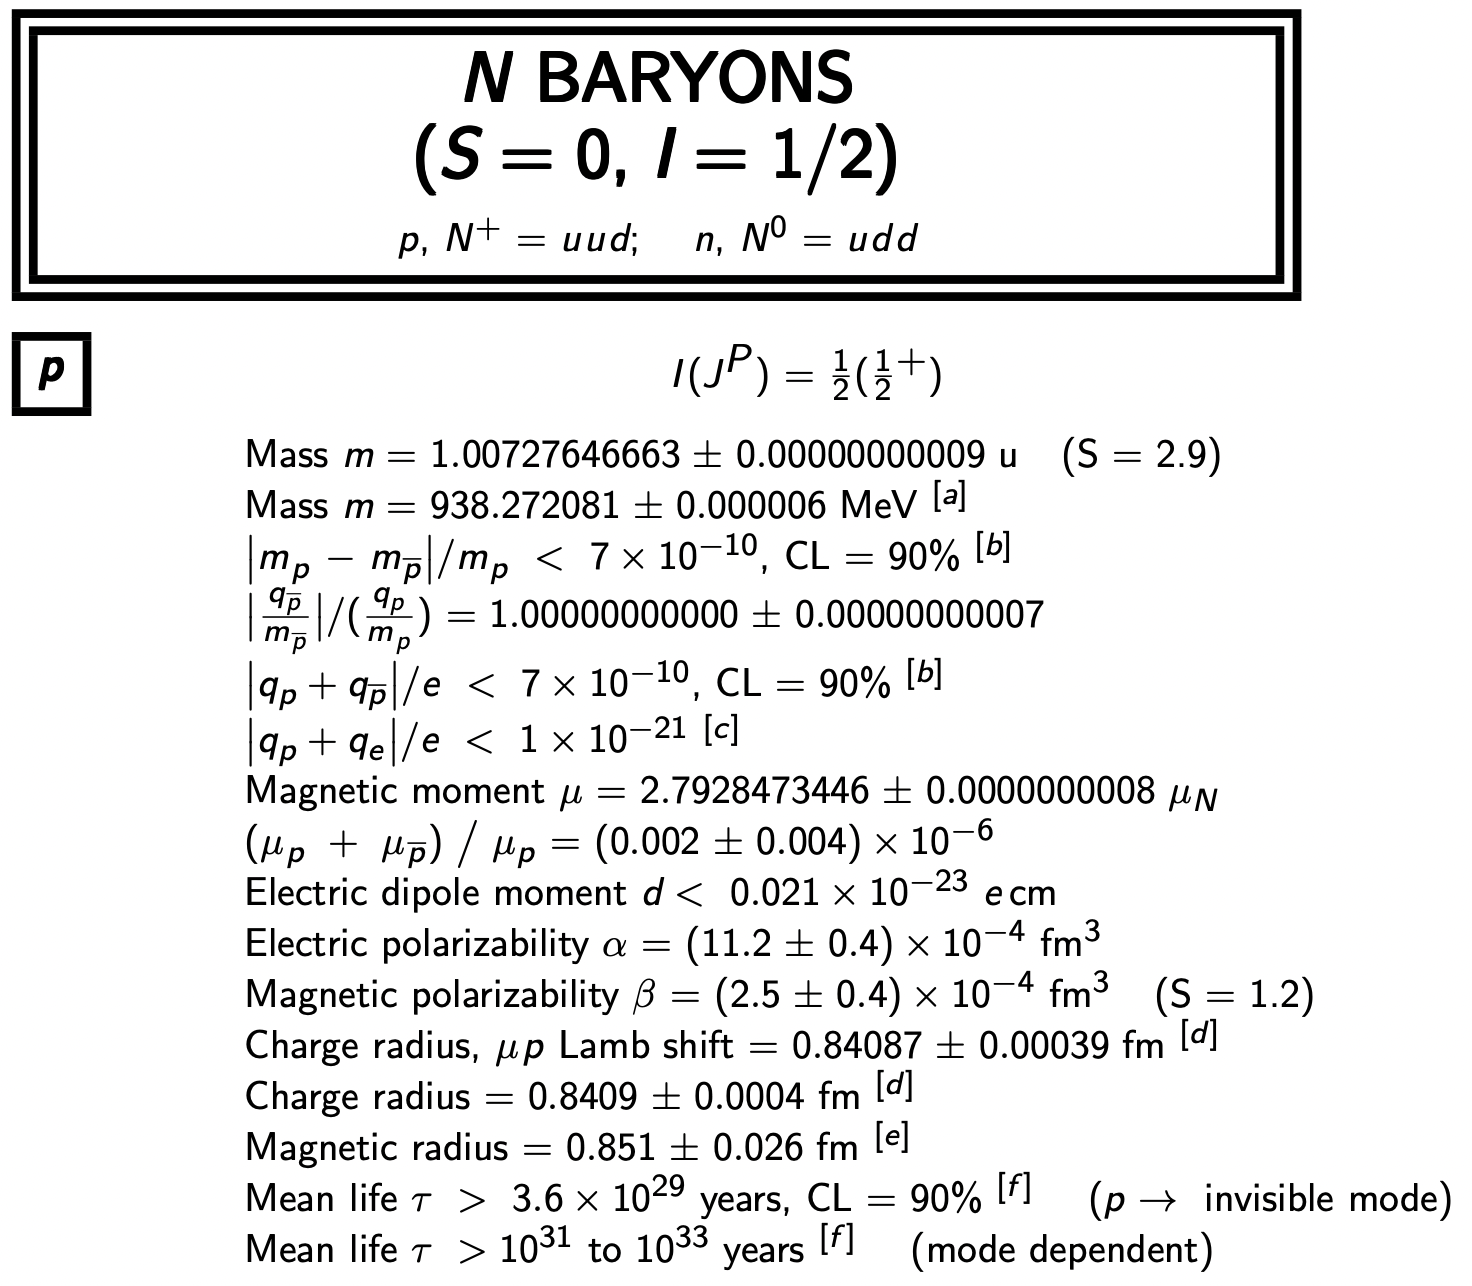
\includegraphics[width=0.8\textwidth]{PDG/N_BARYONS_AND_PROTON.png}
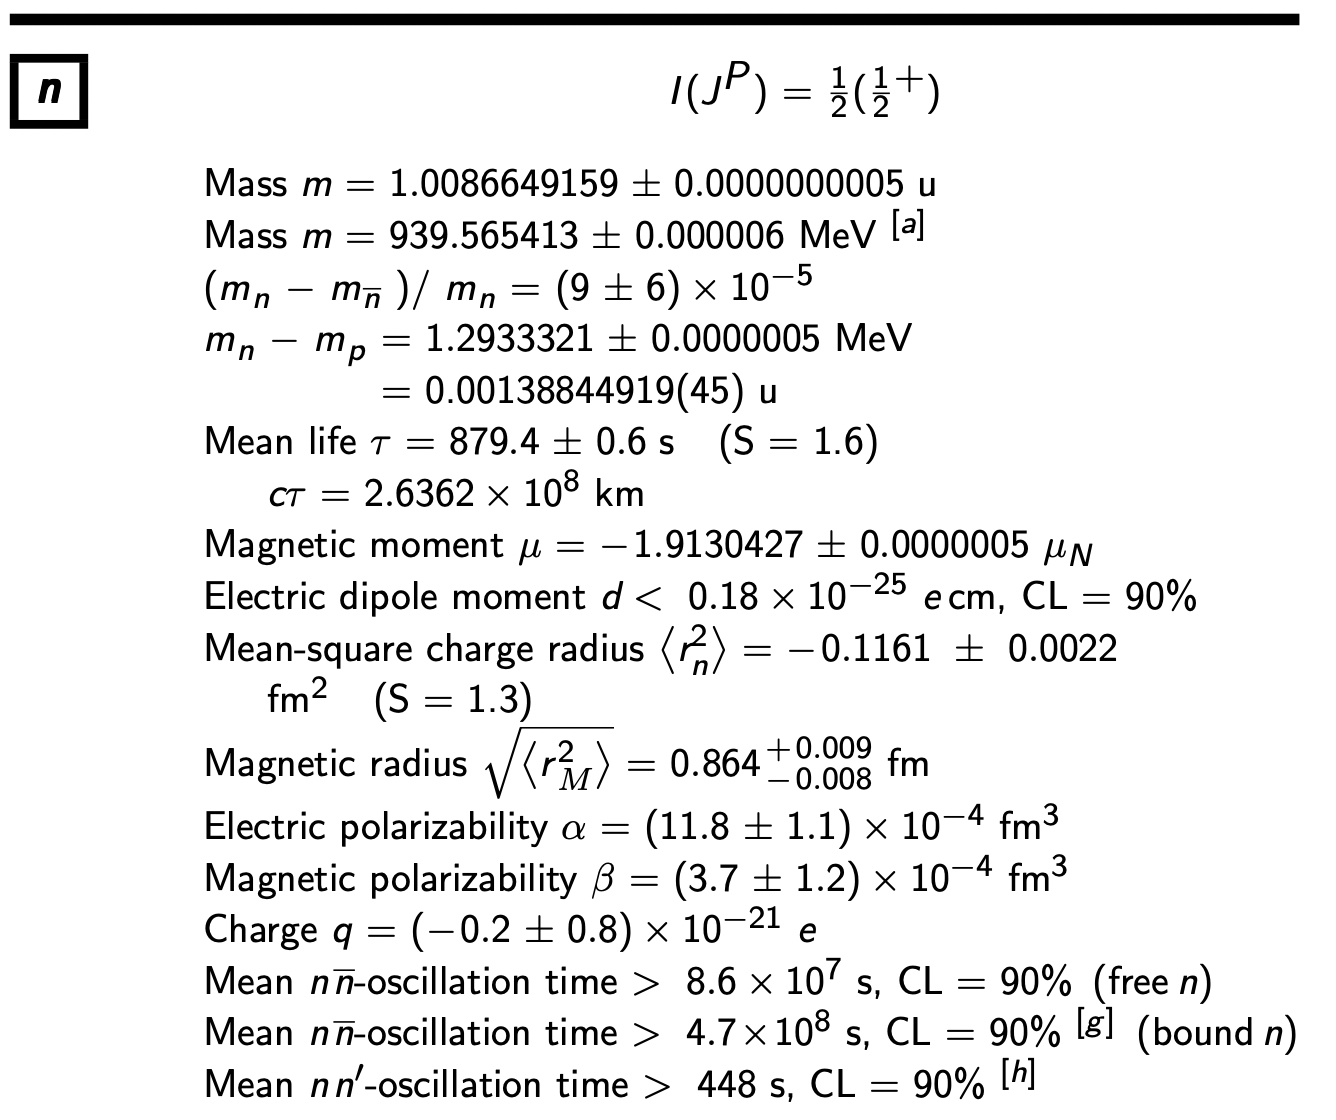
\includegraphics[width=0.8\textwidth]{PDG/neutron.png}
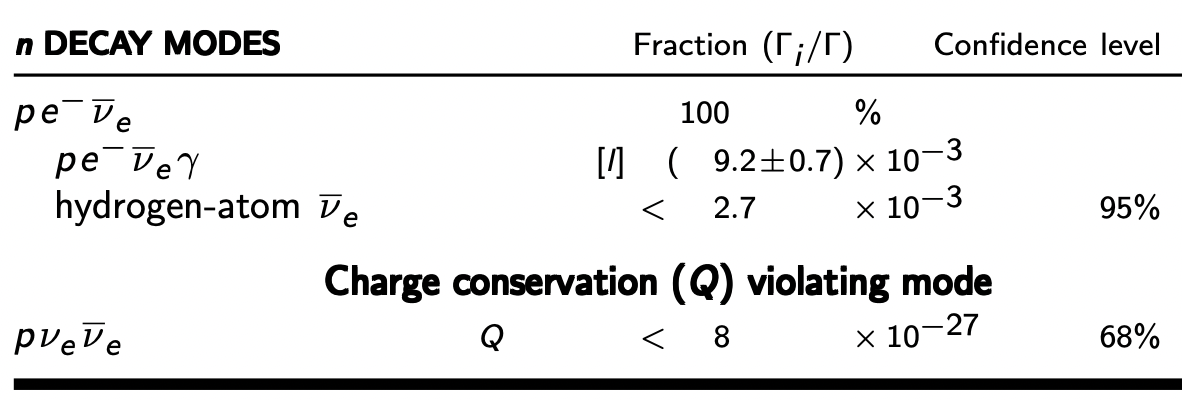
\includegraphics[width=0.8\textwidth]{PDG/neutron_DECAY_MODES.png}
%\clearpage
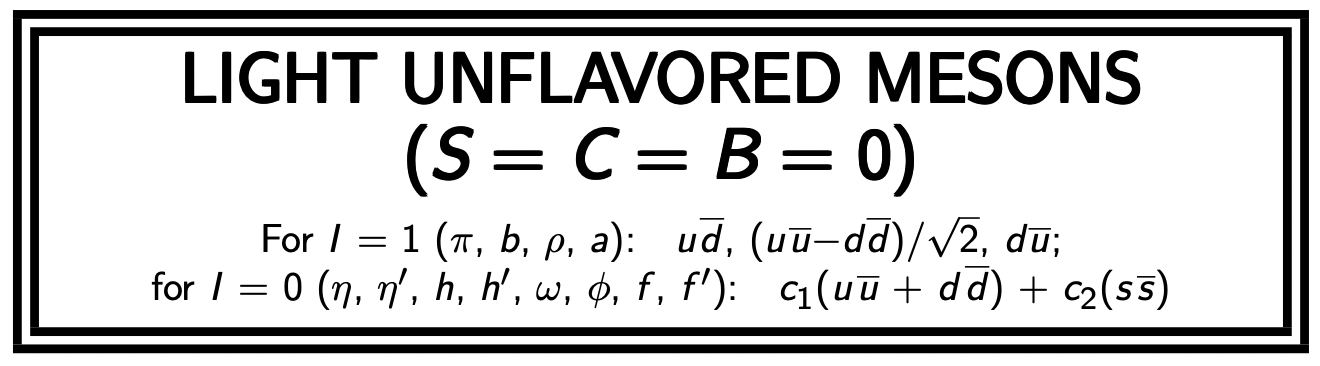
\includegraphics[width=0.8\textwidth]{PDG/LIGHT_UNFLAVOURED_MESONS.png}
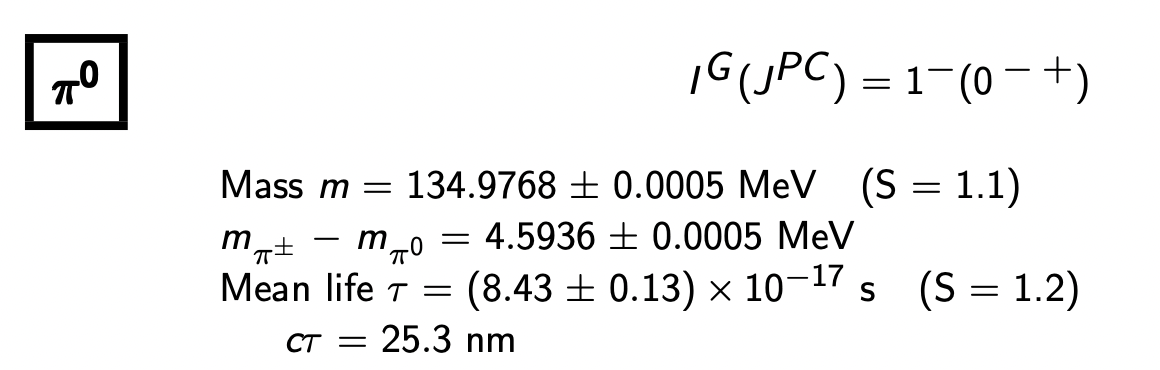
\includegraphics[width=0.8\textwidth]{PDG/PI_ZERO.png}
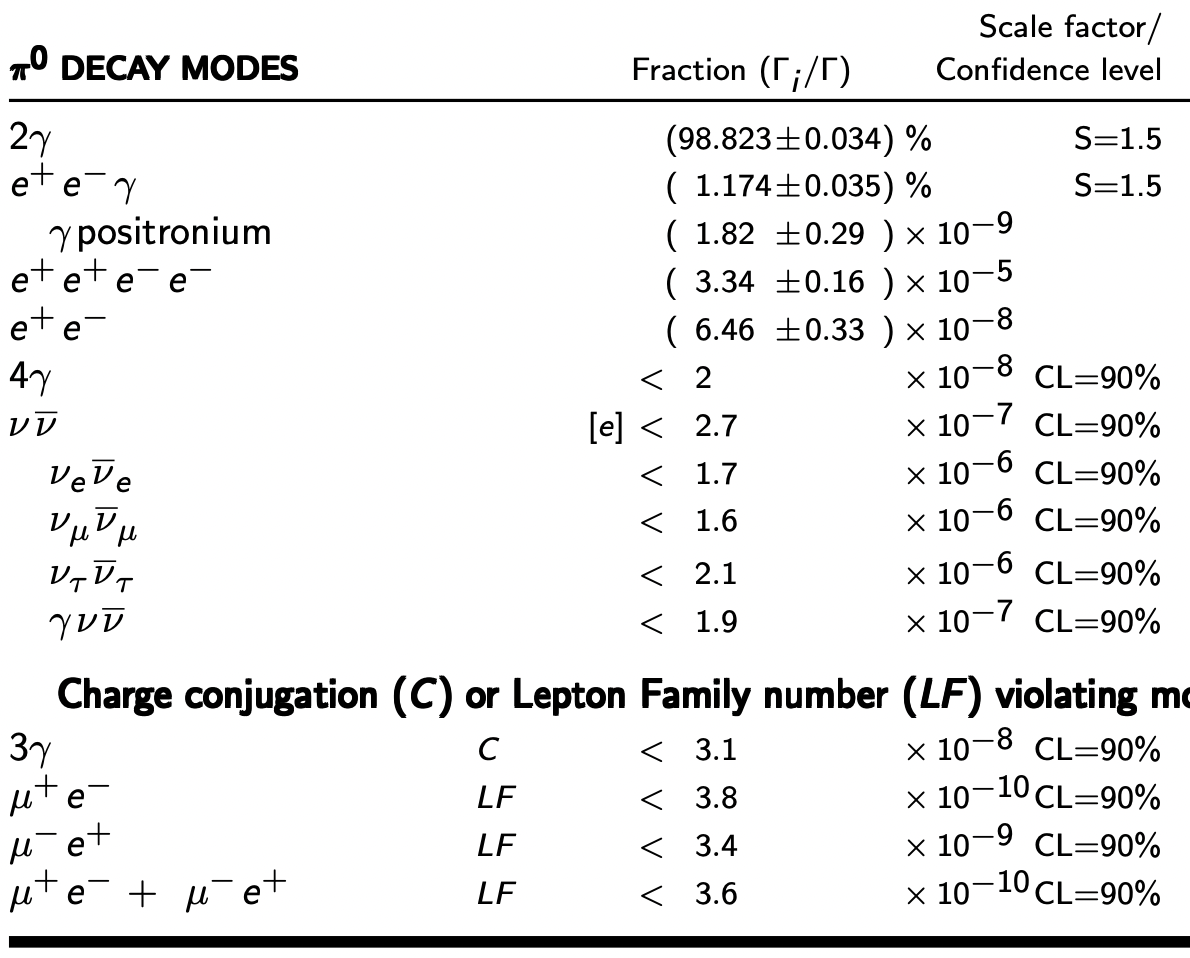
\includegraphics[width=0.8\textwidth]{PDG/PI_ZERO_DECAYS.png}
\clearpage
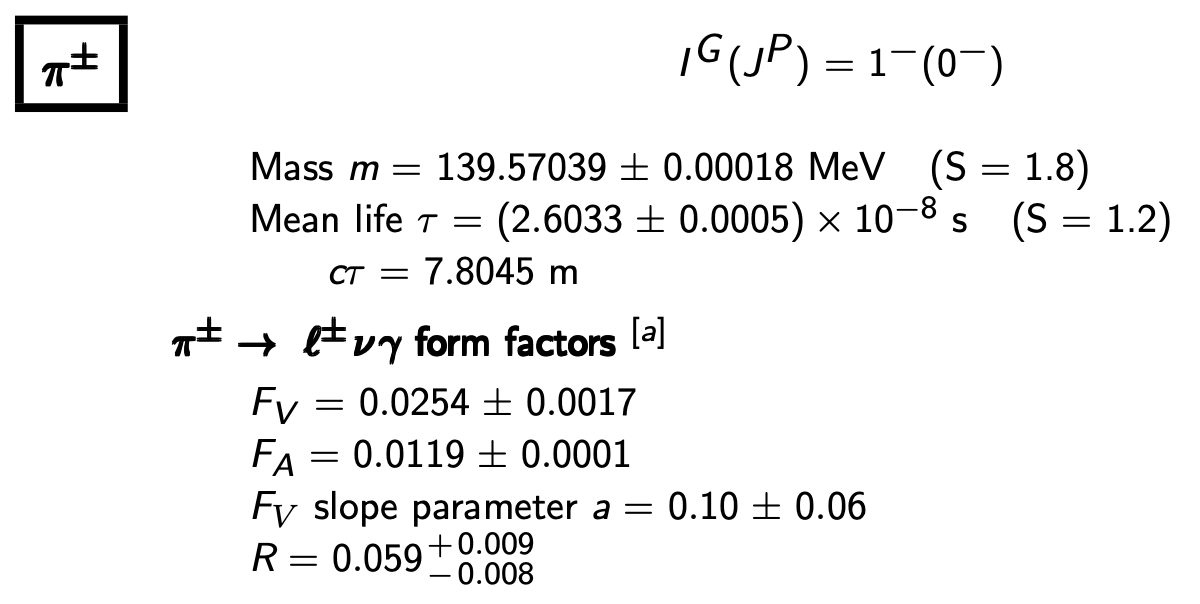
\includegraphics[width=0.8\textwidth]{PDG/PI_PLUS.png}
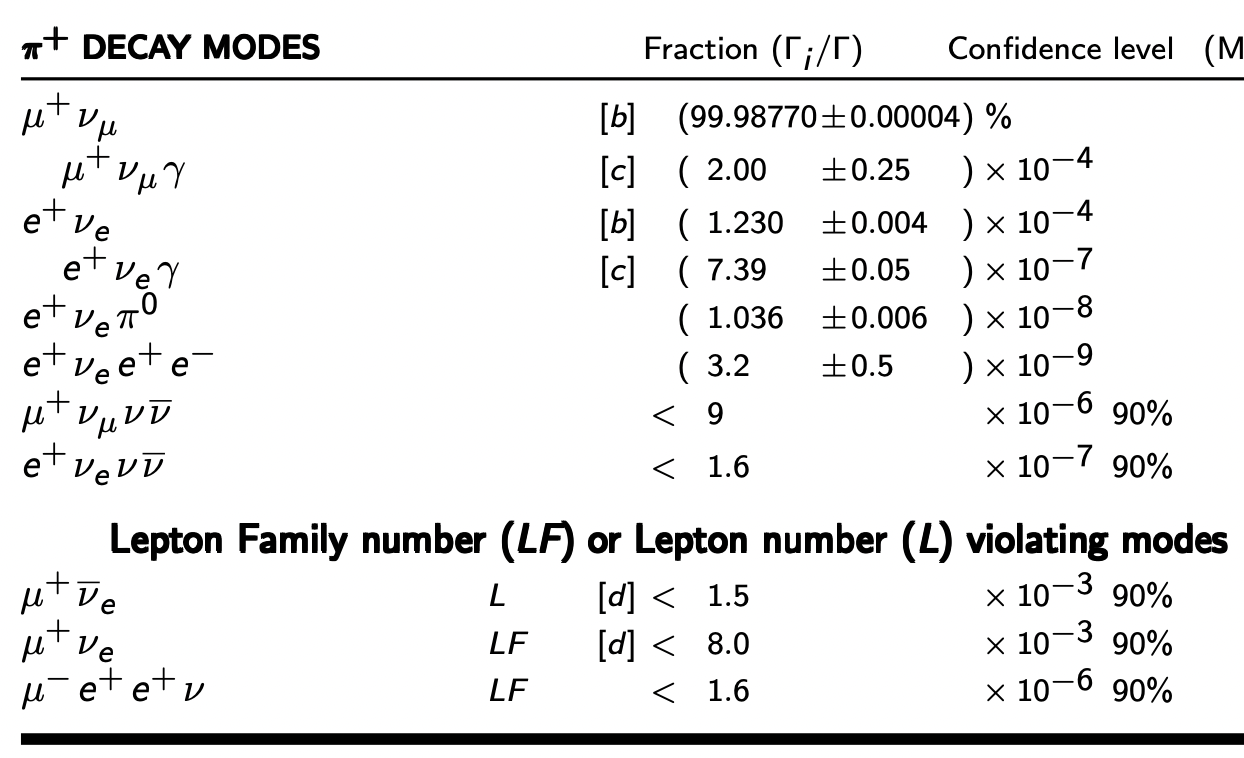
\includegraphics[width=0.8\textwidth]{PDG/PI_PLUS_DECAYS.png}
%\clearpage
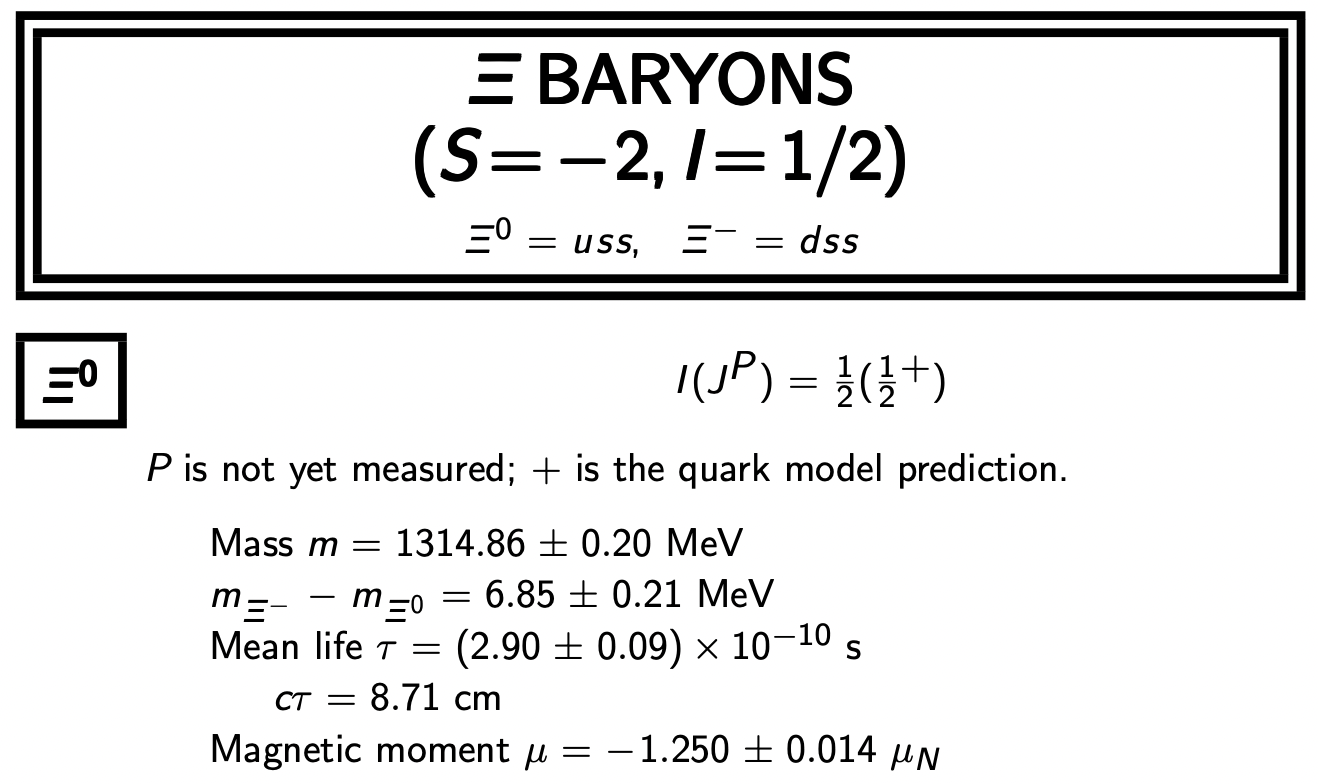
\includegraphics[width=0.8\textwidth]{PDG/XI_BARYONS.png}
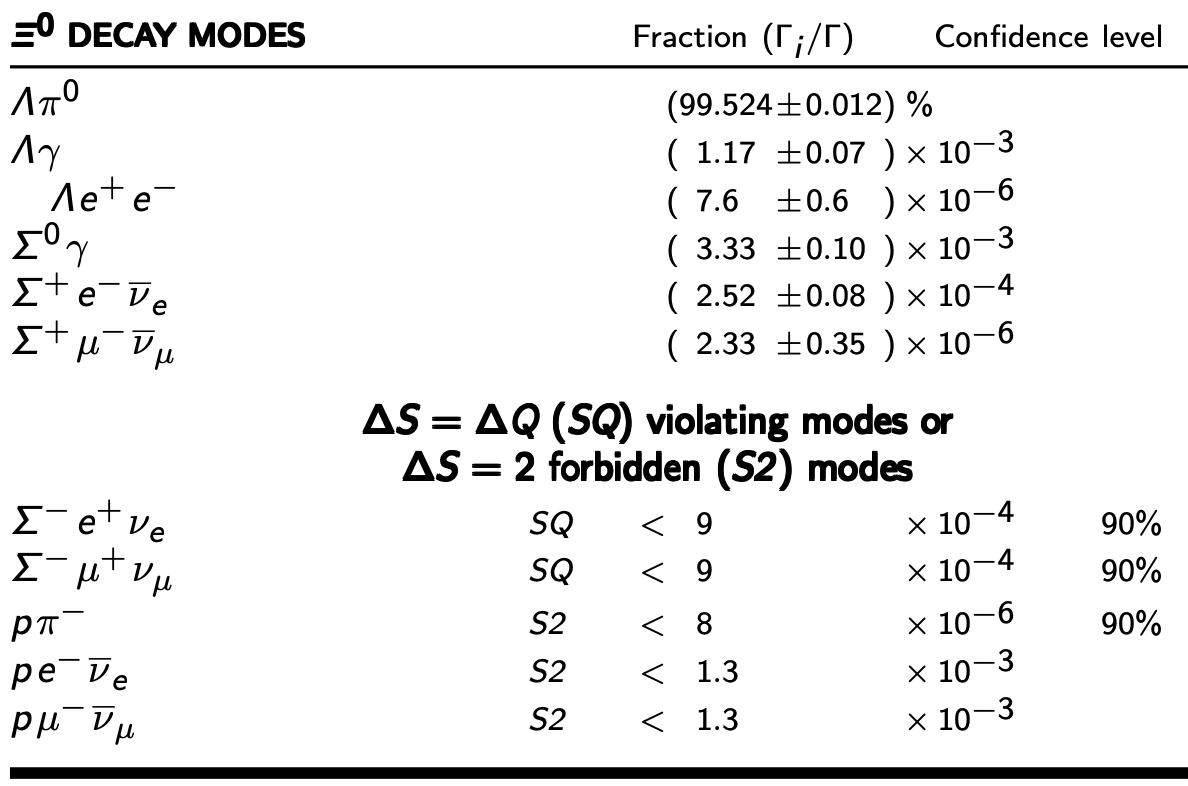
\includegraphics[width=0.8\textwidth]{PDG/XI_DECAY_MODES.png}
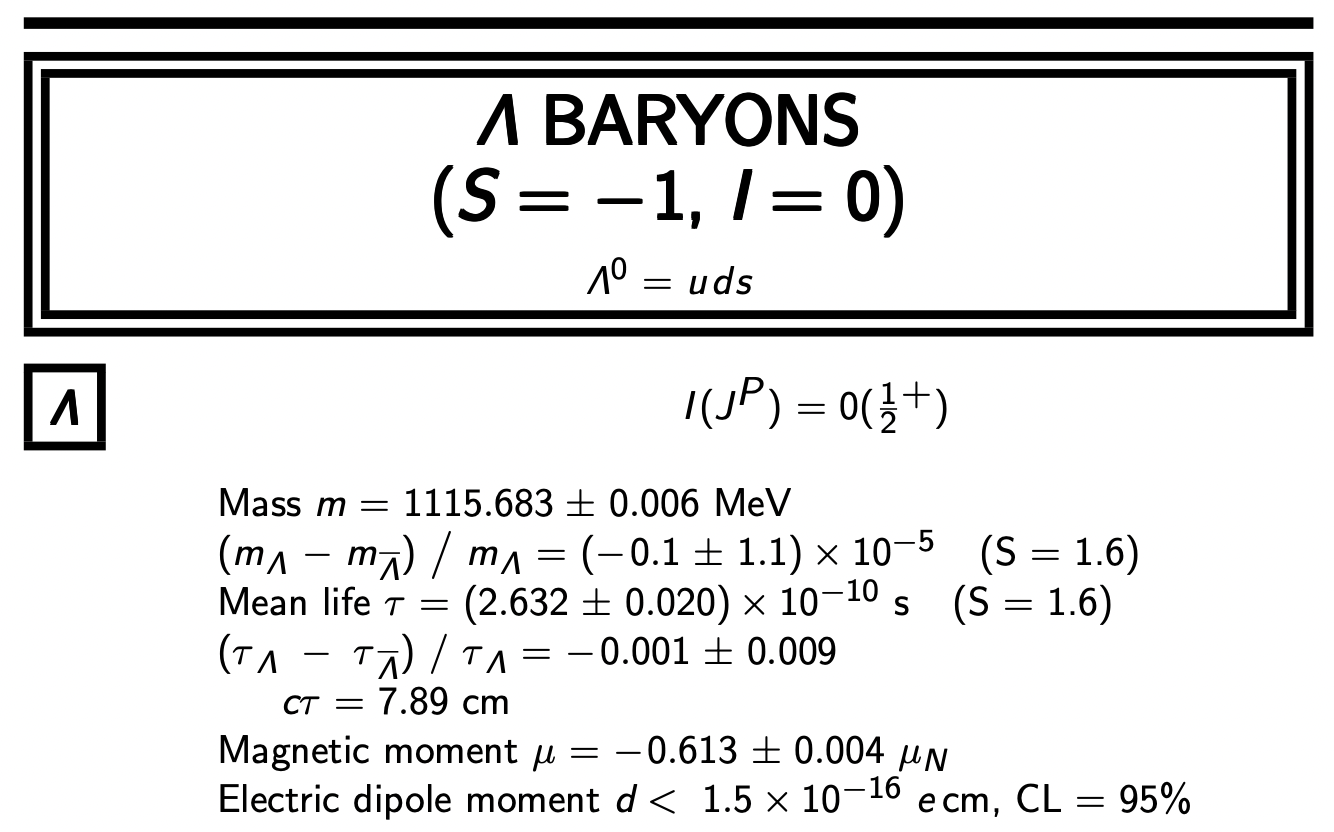
\includegraphics[width=0.8\textwidth]{PDG/LAMBDA_BARYONS.png}
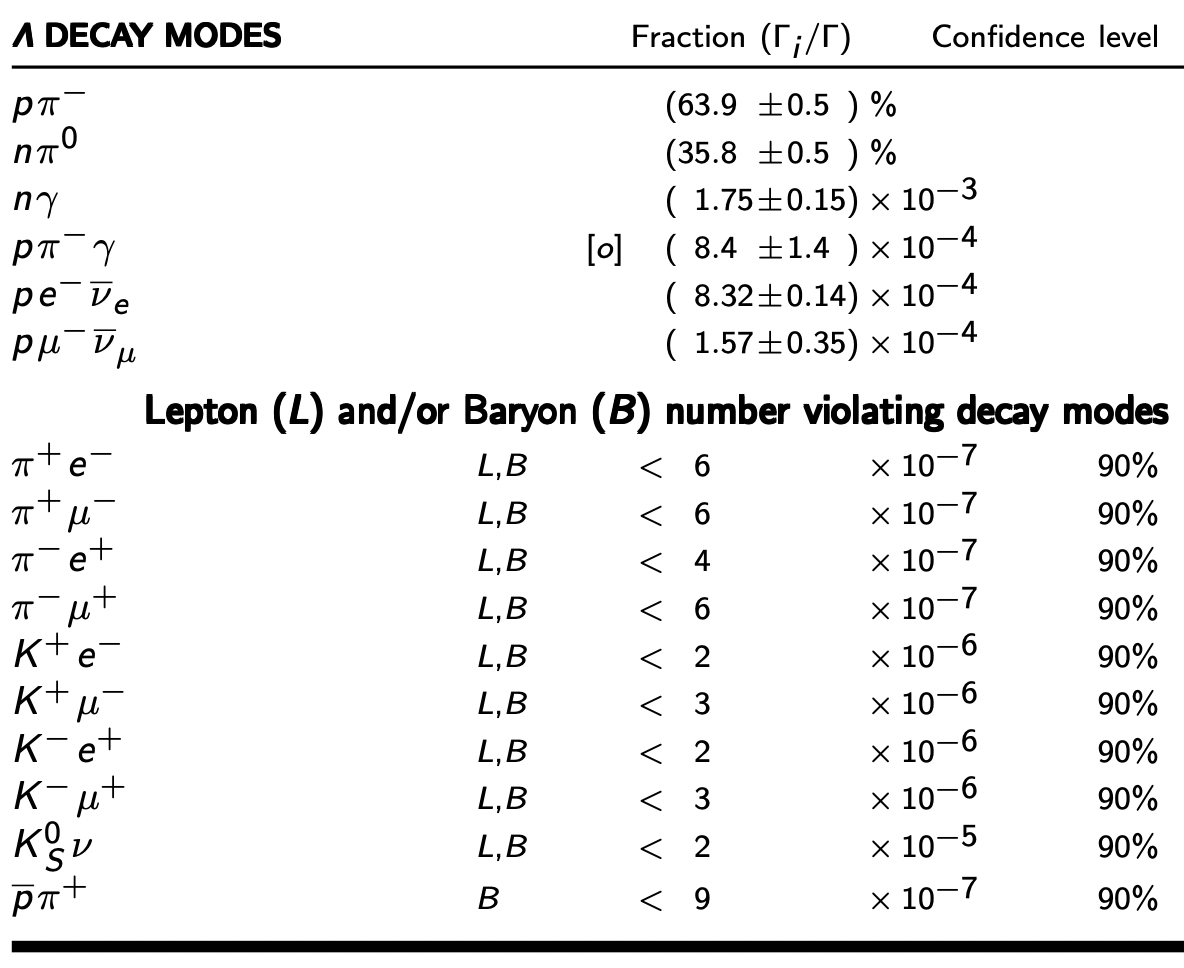
\includegraphics[width=0.8\textwidth]{PDG/LAMBDA_DECAY_MODES.png}
\end{center}

\end{questions}

\endofpaper
\end{document}

